\def\ShowRevisions{1}
\documentclass[remotesensing,article,submit,moreauthors]{Definitions/mdpi}

% The MDPI class already loads the mathematics, table, graphics, float,
% caption, color, list, citation, hyperlink, URL, and microtype packages used
% by this manuscript. Only xspace is additional here.
\usepackage{xspace}

% Toggle this flag in the marked copy. The clean manuscript keeps revised
% passages black while the response-package copy renders them in red.
\newif\ifshowrevisions
\ifdefined\ShowRevisions
  \showrevisionstrue
\else
  \showrevisionsfalse
\fi
\ifshowrevisions
  \newcommand{\revised}[1]{\textcolor{red}{#1}}
  \newenvironment{revisedblock}{\color{red}}{}
\else
  \newcommand{\revised}[1]{#1}
  \newenvironment{revisedblock}{}{}
\fi

\definecolor{cbadred}{HTML}{C0392B}
\definecolor{modelblue}{HTML}{2874A6}
\definecolor{softgray}{HTML}{F3F5F7}
\newcommand{\R}{\mathbb{R}}
\DeclareMathOperator{\clip}{clip}

% Generated numerical macros must be available to the MDPI front matter.
\newcommand{\PhysicalCBADMinPct}{0.45\%\xspace}
\newcommand{\PhysicalCBADMaxPct}{0.85\%\xspace}
\newcommand{\SensitivityMinPct}{0.50\%\xspace}
\newcommand{\SensitivityMaxPct}{1.66\%\xspace}
\newcommand{\PhysicalCorrDataWork}{0.660\xspace}
\newcommand{\MPCNominalPlanningMs}{4.82\xspace}
\newcommand{\MPCNominalCost}{90.83\xspace}
\newcommand{\PhysicalNominalDQNCost}{78.33\xspace}
\newcommand{\PhysicalNominalCBADCost}{77.66\xspace}
\newcommand{\PhysicalAuditTasks}{20,000\xspace}
\newcommand{\IndependentModelSeeds}{20\xspace}
\newcommand{\PrimaryHolmPMax}{0.08278\xspace}
\newcommand{\PrimarySupportedCount}{3\xspace}
\newcommand{\PrimaryNegativeSeedsMin}{15\xspace}
\newcommand{\PrimaryNegativeSeedsMax}{17\xspace}
\newcommand{\LateCBADCost}{80.36\xspace}
\newcommand{\LateDQNCost}{81.06\xspace}
\newcommand{\LateCBADEnergy}{1.50\xspace}
\newcommand{\LateDQNEnergy}{1.50\xspace}
\newcommand{\LateCBADLatency}{16.52\xspace}
\newcommand{\LateDQNLatency}{16.60\xspace}
\newcommand{\LateCBADPenalty}{51.34\xspace}
\newcommand{\LateDQNPenalty}{51.80\xspace}
\newcommand{\MismatchHolmPMax}{0.5264\xspace}
\newcommand{\MismatchLowHolmPMax}{0.5264\xspace}
\newcommand{\MismatchLowSupportedCount}{3\xspace}
\newcommand{\MismatchHighHolmPMax}{0.2632\xspace}
\newcommand{\MismatchHighSupportedCount}{3\xspace}

\newcommand{\FullQDifference}{-0.19\xspace}
\newcommand{\FullQHolmP}{0.05909\xspace}
\newcommand{\CenteredDifference}{-0.48\xspace}
\newcommand{\CenteredCILow}{-0.96\xspace}
\newcommand{\CenteredCIHigh}{-0.10\xspace}
\newcommand{\CenteredHolmP}{0.7895\xspace}
\newcommand{\ImmediateDifference}{-0.49\xspace}
\newcommand{\ImmediateHolmP}{1\xspace}
\newcommand{\BootstrapDifference}{-0.18\xspace}
\newcommand{\BootstrapCILow}{-0.49\xspace}
\newcommand{\BootstrapCIHigh}{0.11\xspace}
\newcommand{\BootstrapHolmP}{1\xspace}
\newcommand{\DoubleDifference}{-0.67\xspace}
\newcommand{\DoubleCILow}{-1.18\xspace}
\newcommand{\DoubleCIHigh}{-0.24\xspace}
\newcommand{\DoubleHolmP}{0.03545\xspace}
\newcommand{\FullQSupportedCount}{0\xspace}
\newcommand{\CBADSupportedCount}{3\xspace}
\newcommand{\CenteredSupportedCount}{0\xspace}
\newcommand{\ImmediateSupportedCount}{0\xspace}
\newcommand{\BootstrapSupportedCount}{0\xspace}
\newcommand{\DoubleSupportedCount}{3\xspace}
\newcommand{\DQNFamilyNominalMinCost}{77.66\xspace}
\newcommand{\DQNFamilyNominalMaxCost}{78.40\xspace}
\newcommand{\DQNFamilyBelowMPCCount}{30\xspace}
\newcommand{\PlannerCostHOne}{99.33\xspace}
\newcommand{\PlannerTimeHOne}{0.13\xspace}
\newcommand{\PlannerCostHTwo}{92.80\xspace}
\newcommand{\PlannerTimeHTwo}{0.50\xspace}
\newcommand{\PlannerCostHFour}{90.83\xspace}
\newcommand{\PlannerTimeHFour}{4.82\xspace}
\newcommand{\PlannerCostHSix}{89.35\xspace}
\newcommand{\PlannerTimeHSix}{42.50\xspace}

\newcommand{\DQNvsMPCContrastCount}{30\xspace}
\newcommand{\DQNvsMPCSupportedCount}{30\xspace}
\newcommand{\DQNvsMPCGlobalWorstDifference}{-5.92\xspace}
\newcommand{\DQNvsMPCGlobalUpperBound}{-5.03\xspace}
\newcommand{\DQNvsMPCHolmPMax}{5.722e-05\xspace}
\newcommand{\DQNvsMPCNegativeSeedMin}{20\xspace}
\newcommand{\DQNvsMPCNegativeSeedMax}{20\xspace}


% MDPI internal metadata; dates are assigned during editorial processing.
\firstpage{1}
\makeatletter
\setcounter{page}{\@firstpage}
\makeatother
\pubvolume{1}
\issuenum{1}
\articlenumber{0}
\pubyear{2026}
\copyrightyear{2026}
\datereceived{ }
\daterevised{ }
\dateaccepted{ }
\datepublished{ }

\Title{Statistical Evidence for a DQN-Family Advantage in a Resource-Coupled Satellite-Ground Scheduling Benchmark}

\Author{Bocheng Yang $^{1}$, Lujie Zheng $^{1}$, Dingyang Lyu $^{3}$, Jian Liu $^{1,2,*}$ and Bo Chen $^{1,*}$}
\AuthorNames{Bocheng Yang, Lujie Zheng, Dingyang Lyu, Jian Liu and Bo Chen}

\address{%
$^{1}$ \quad School of Aerospace, Harbin Institute of Technology, Shenzhen 518055, China; 25b961001@stu.hit.edu.cn (B.Y.); 24s061021@stu.hit.edu.cn (L.Z.);\\
$^{2}$ \quad Guangxi Key Laboratory of Precision Navigation Technology and Application, Guilin University of Electronic Technology, Guilin 541004, China;\\
$^{3}$ \quad Zhongguancun Academy, Beijing 100094, China; s-ldy25@bza.edu.cn (D.L.)}

% Two corresponding authors are retained at the authors' explicit request.
\corres{Correspondence: hitchenbo@hit.edu.cn (B.C.); liujian2024@hit.edu.cn (J.L.)}

\abstract{\revised{Resource-coupled satellite-ground scheduling requires decisions with computational, energy, thermal, and communication effects that persist across task arrivals. We tested whether the deep Q-network (DQN) family provides a reproducible advantage over short-horizon planning in a synthetic benchmark with clipped, soft-constrained resources. Six DQN objectives used the same state representation, network architecture, replay procedure, optimizer, interaction budget, \IndependentModelSeeds{} model seeds, and held-out traces. We evaluated them across five fully coupled regimes. In all \DQNvsMPCContrastCount{} objective--regime comparisons, the mean episode cost for each DQN objective was lower than that of four-step model-predictive control (MPC-4). Every paired 95\% bootstrap interval excluded zero, and all Holm-adjusted sign tests supported the same ordering. The least-favorable mean difference was \DQNvsMPCGlobalWorstDifference, and the family-wide simultaneous 95\% upper bound was \DQNvsMPCGlobalUpperBound. Differences among DQN objectives were smaller and scenario dependent. Additional nominal tests quantify discount-factor, training-length, greedy-rollout, and CPU decision-time sensitivity. These findings describe this synthetic soft-constraint benchmark only; hard energy and thermal limits can change the feasible action set and therefore the algorithm ordering.}}

\keyword{deep Q-network variants; satellite edge computing; task scheduling; model-assisted reinforcement learning; full-action supervision}

\addhighlights{yes}
\renewcommand{\addhighlights}{%
\par\vspace{6pt}\noindent
\textbf{What are the main findings?}
\begin{itemize}[labelsep=2.5mm,topsep=-3pt]
\item All \DQNvsMPCContrastCount{} paired DQN--MPC-4 objective--regime comparisons supported a DQN-family advantage.
\item Within-family differences were smaller and scenario dependent, while deeper exact planning reduced cost but required substantially more decision time.
\end{itemize}\vspace{3pt}
\textbf{What are the implications of the main findings?}
\begin{itemize}[labelsep=2.5mm,topsep=-3pt]
\item \revised{Long-horizon value learning can outperform short-horizon planning in this synthetic, clipped-resource, soft-constrained benchmark.}
\item \revised{The benchmark is a reproducible testbed for future hard-constraint, mission-calibrated, and operational validation.}
\end{itemize}
}

\begin{document}
\emergencystretch=2em

\begin{figure}[H]
\centering
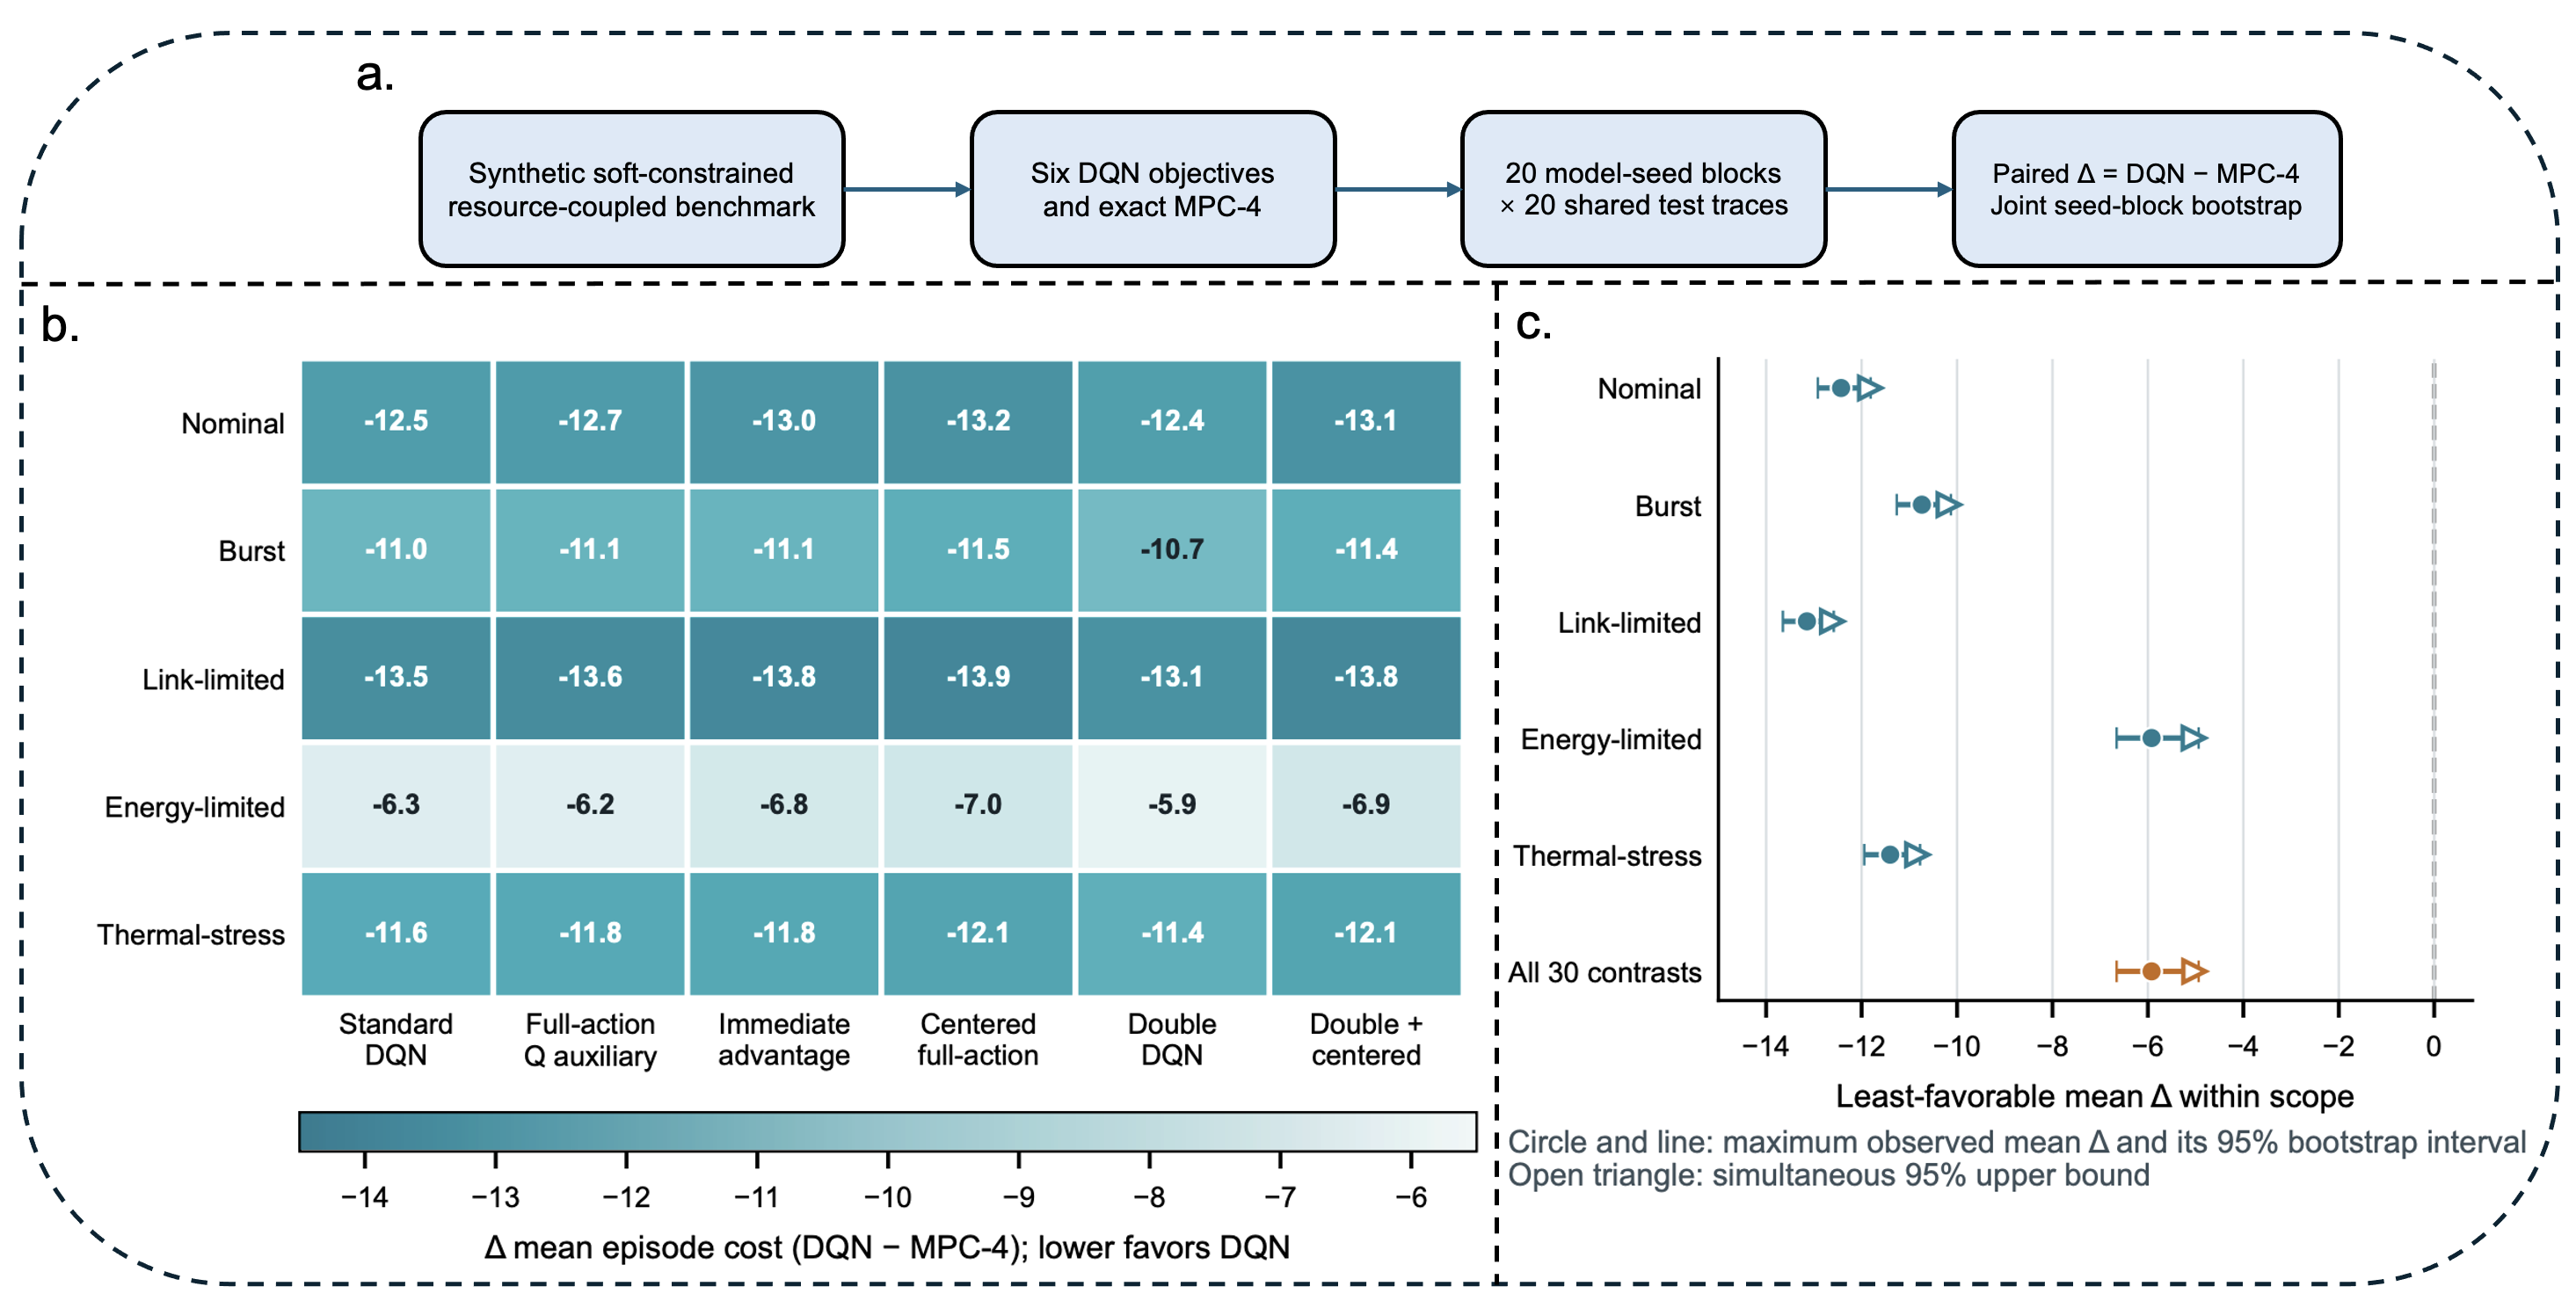
\includegraphics[width=0.98\textwidth,height=0.45\textheight,keepaspectratio]{fig1.jpg}
\caption{Family-level evidence for deep Q-network (DQN) methods relative to four-step model-predictive control (MPC-4) in the synthetic benchmark with soft constraints. (a) The evaluation uses 20 paired model-seed blocks, each averaging 20 shared held-out traces. (b) Cells report the mean episode-cost difference between each DQN objective and MPC-4; negative values favor DQN. (c) Circles and lines show the largest, least-favorable mean difference within each scope and its 95\% joint-bootstrap interval. Open triangles show simultaneous 95\% upper bounds. A single 10,000-resample seed-block bootstrap preserves correlation among the 30 contrasts. Exact two-sided sign tests are Holm-adjusted across all comparisons, which satisfy the prespecified support rule.}
\label{fig:graphical}
\end{figure}

\section{Introduction}

Earth-observation and communication satellites increasingly execute perception and decision workloads in orbit. Compact onboard networks can reduce downlink demand and response latency under constrained computational resources~\cite{9925218,10107454,10378728,10440355,10423050}. Onboard execution consumes heat, energy, and computing capacity, whereas ground offloading consumes contact time and bandwidth. Scheduling must therefore coordinate onboard execution, complete offloading, and collaborative preprocessing over time.

Existing schedulers optimize constellation coordination, observation plans, service placement, deadlines, makespan, or energy use~\cite{RN8,RN10,RN20,RN22,RN23,RN27,RN28}. In our setting, every decision changes six resources that persist across task arrivals: heat, energy, queue occupancy, compute utilization, bandwidth, and remaining contact time. An action with a low immediate cost can therefore restrict the choices available for later tasks. This temporal coupling raises a central question: can learned long-horizon values outperform transparent one-step and finite-horizon alternatives across changing resource conditions?

\begin{revisedblock}
Operational optimization faces two linked difficulties. Exact mixed-integer or dynamic-programming formulations require a calibrated transition model and grow rapidly with tasks, resource states, and horizon; receding-horizon control additionally depends on forecasts that must be recomputed within the onboard decision budget. Learned policies shift most computation offline and provide fast direct actions, but they replace online optimization guarantees with dependence on the training distribution. Our benchmark isolates this trade-off under a small discrete action set and a fully inspectable simulator rather than resolving it for flight operations.

Standard deep Q-network (DQN) learning~\cite{mnih2015human,watkins1992q} constructs one Bellman target from each factual tuple $(s_t,a_t,r_t,s_{t+1})$. In our setting, analytical resource equations can also evaluate every unexecuted action without advancing the environment or revealing later tasks. This structure enables controlled evaluation of the DQN family and alternative uses of full-action supervision during training.

The distinction between the present simulator and an operational scheduler is central. Here, energy, heat, queue, bandwidth, and contact states are clipped and over-limit exposure contributes a penalty while the episode continues. Real spacecraft generally enforce hard energy and thermal envelopes through action inhibition, task rejection, or protective shutdown. A hard constraint changes the feasible action set and can make a policy with a lower penalized cost infeasible. Consequently, the ordering observed below is a statement about the specified soft-constraint benchmark and cannot be transferred directly to an on-orbit controller.
\end{revisedblock}

We compare six DQN objectives: standard DQN, full-action Q, immediate advantage, centered full-action, Double DQN, and Double DQN with centered full-action supervision. A separate $\gamma=0$ contextual bandit provides a learned one-step comparator. Model-evaluated alternatives are used only during training. During evaluation and deployment, every policy acts directly from its learned Q-values.

We make three contributions:

\begin{enumerate}[leftmargin=1.6em]
    \item We introduce a fully specified, reproducible benchmark that links task primitives to three processing pathways and six persistent computational, energy, thermal, and communication resources.
    \item We construct a controlled six-objective DQN family that varies factual supervision, full-action targets, centering, bootstrapping, and Double DQN evaluation under matched training conditions.
    \item We test the family-level result against four-step model-predictive control (MPC-4) through \DQNvsMPCContrastCount{} paired objective--regime contrasts, a correlation-preserving joint bootstrap, multiplicity-corrected tests, and a simultaneous upper bound.
\end{enumerate}

\section{Related Work and Study Positioning}

\subsection{Satellite-ground scheduling}

Satellite schedulers address constellation coordination, observation planning, service placement, and energy-aware offloading~\cite{RN8,RN10,RN20,RN22,RN23,RN27,RN28}. Our setting combines an explicit cost for every action with resource carryover between task arrivals. Because each immediate action cost is directly evaluable, the one-step objective is observable. The benchmark therefore asks whether a learned value function can exploit consequences that persist beyond this immediate cost.

\begin{revisedblock}
Classical optimization remains an important comparator frontier. Mixed-integer linear programming can encode coupled observation and resource constraints and can provide exact or bounded solutions on instances of manageable size~\cite{chen2019milp}. Dynamic programming and exact decomposition exploit temporal structure for smaller or specially structured instances~\cite{peng2020exact}. PPO~\cite{schulman2017ppo} and discrete-action adaptations of SAC~\cite{haarnoja2018sac} provide alternative policy-learning baselines with different stability and exploration trade-offs. These methods may outperform DQN when hard feasibility, continuous controls, or stronger global look-ahead dominates; they were not implemented in this revision, so the present study does not claim universal DQN optimality.
\end{revisedblock}

\subsection{Model use and full-action learning}

Dyna introduced simulated experience for value learning and planning~\cite{sutton1991dyna}. Fitted dynamics can likewise accelerate deep Q-learning~\cite{gu2016continuous}. Counterfactual data fusion and causal augmentation construct transitions under structural assumptions~\cite{forney2017counterfactual,armengol2024caiac}. Counterfactual credit assignment instead separates action influence from future randomness~\cite{mesnard2021counterfactual}. Recent work has also examined multi-action generative interfaces and joint quantities across action outcomes~\cite{kaya2026joint}. Together, these studies provide several routes for incorporating modeled alternatives into reinforcement learning.

Advantage learning modifies Bellman operators to widen action gaps~\cite{bellemare2016gap}. Four objectives in our DQN family instead retain their respective Bellman target rules while adding modeled outcomes for all actions at a sampled state. Table~\ref{tab:closest_methods} positions this training-time supervision interface relative to related mechanisms. Standard DQN and Double DQN serve as factual-only family controls. We compare the DQN family with short-horizon planning and examine how target construction, centering, and target evaluation affect within-family variation.

In this manuscript, ``counterfactual'' denotes a model-evaluated one-step outcome for an unexecuted action under the same current task and exogenous state. It does not denote an identified causal effect from observational data.

\begin{table}[H]
\centering
\caption{Positioning of training-time modeled-action supervision used by four deep Q-network (DQN) objectives. ``All actions'' means that one update can use modeled outcomes for every discrete action at the sampled state. Standard DQN and Double DQN provide factual-only family controls.}
\label{tab:closest_methods}
\small
\setlength{\tabcolsep}{4pt}
\begingroup
\renewcommand\tabularxcolumn[1]{p{#1}}
\begin{tabularx}{\textwidth}{>{\raggedright\arraybackslash}p{0.24\textwidth}>{\raggedright\arraybackslash}p{0.18\textwidth}>{\raggedright\arraybackslash}p{0.21\textwidth}>{\raggedright\arraybackslash}X}
\toprule
Method family & Source of modeled information & How it enters learning & Relation to the evaluated supervision interface \\
\midrule
Dyna and local model-based acceleration~\cite{sutton1991dyna,gu2016continuous} & Learned or fitted dynamics & Simulated experience or local rollouts & Does not use one simultaneous analytical outcome per action in a training-only auxiliary objective \\
Causal counterfactual augmentation~\cite{armengol2024caiac} & Structural assumptions and offline trajectories & Synthetic transitions augment the training distribution & Targets distributional coverage rather than within-state Bellman action gaps \\
Counterfactual credit assignment~\cite{mesnard2021counterfactual} & Future-conditioned trajectory information & Policy-gradient baseline or critic & Model-free and trajectory-conditioned rather than analytical one-step action enumeration \\
Joint Markov decision processes (MDPs)~\cite{kaya2026joint} & Multi-action sample transition model & Joint action-outcome quantities and Bellman operators & Closest formal interface; not a training-only auxiliary objective on a fixed factual DQN backbone \\
Evaluated full-action DQN objectives & Deterministic analytical one-step transition for three actions & Auxiliary full-action targets or centered action gaps; no replay insertion & One controlled factor within a six-objective family; the family claim also includes factual-only controls \\
\bottomrule
\end{tabularx}
\endgroup
\end{table}

\section{Materials and Methods}

\subsection{System Model and Immediate-Cost Quantification}
\label{sec:system}

At each task arrival $t$, a satellite selects one of three actions. Action $\alpha_s$ executes the task onboard and downlinks the result, whereas $\alpha_g$ downlinks the complete input for ground execution. Action $\alpha_{s\&g}$ performs onboard preprocessing followed by ground execution:
\begin{equation}
\mathcal A=\{\alpha_s,\alpha_g,\alpha_{s\&g}\},
\end{equation}
where the subscripts denote satellite, ground, and collaborative processing, respectively.

\begin{figure}[H]
\centering
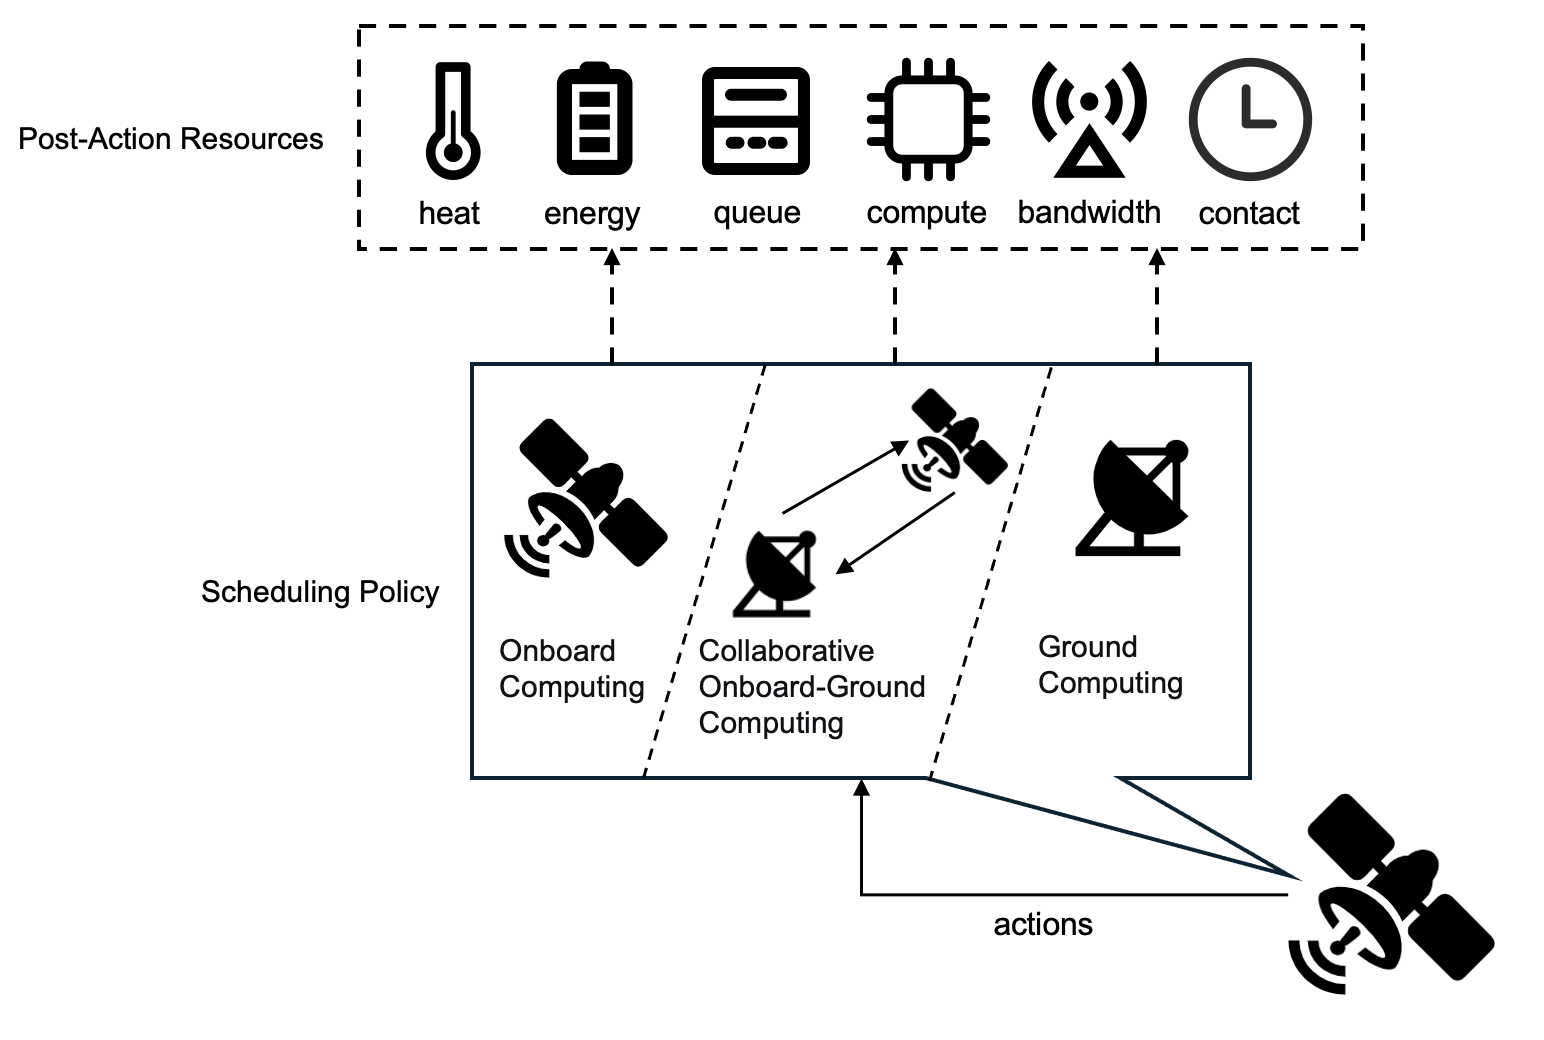
\includegraphics[width=0.98\textwidth,height=0.42\textheight,keepaspectratio]{fig2.jpg}
\caption{Three satellite-ground processing pathways. Each arriving task is executed onboard, transferred for ground execution, or preprocessed collaboratively before ground completion. The analytical transition model returns the immediate cost and the post-action heat, energy, queue occupancy, compute utilization, bandwidth, and remaining contact.}
\label{fig:system}
\end{figure}

\subsubsection{Implemented immediate-cost model}

The experiments use the dimensionless linear cost implemented in the internally consistent synthetic simulator. Let $x_k$ denote the 15 task descriptors in Table~\ref{tab:state_dictionary}. Each descriptor is normalized as
\begin{equation}
\bar x_k=\clip(x_k/s_k,0,1.5),
\end{equation}
where $s_k$ is the corresponding scale. For inherited normalized bandwidth $b$, the available return rate is $R(b)=2.2+217.8b$ Mbit s$^{-1}$. The three action latencies are
\begin{align}
L_s&=x_3+1000x_6/R(b),\notag\\
L_g&=x_8+1000x_9/R(b),\notag\\
L_{s\&g}&=1000x_{12}/4+x_{13}+1000x_{15}/R(b).
\label{eq:latencies}
\end{align}
The implemented immediate costs are
\begin{align}
c_s^{imm}={}&0.70\bar x_1+0.65\bar x_2+0.00045L_s+0.55\bar x_5
+0.35\bar x_6+0.35h+0.12(1-e),\notag\\
c_g^{imm}={}&0.45\bar x_7+0.00045L_g+0.55\bar x_9
+0.35(0.28-\tau)_+,\notag\\
c_{s\&g}^{imm}={}&0.55(\bar x_{10}+\bar x_{11})+0.55\bar x_{14}
+0.00045L_{s\&g}+0.45\bar x_{15}\notag\\
&+0.18h+0.12q+0.18(0.22-\tau)_+.
\label{eq:implemented_costs}
\end{align}
Here $h$, $e$, $q$, and $\tau$ denote inherited heat, remaining energy, queue occupancy, and contact duration, respectively. The weights are fixed simulator assumptions rather than fitted mission utilities. The same weights are used during training, counterfactual preview, MPC evaluation, and deployment evaluation. Automated tests reconstruct Eq.~\eqref{eq:implemented_costs} from the 15 raw descriptors and compare the resulting costs with all three implementation outputs.

\begin{table}[H]
\centering
\caption{Implemented 15-dimensional task descriptor dictionary. The complete 24-dimensional observation adds normalized time, the sine and cosine of link phase, and six resource coordinates: $h$, $e$, $q$, compute utilization $u$, bandwidth $b$, and contact duration $\tau$.}
\label{tab:state_dictionary}
\resizebox{\textwidth}{!}{\begin{tabular}{llll}
\toprule
Coordinate & Descriptor & Unit & Normalization scale $s_k$ \\
\midrule
$x_1$ & Onboard compute heat & J & 100 \\
$x_2$ & Total workload & GFLOP & 4.8 \\
$x_3$ & Onboard compute time & ms & 1400 \\
$x_4$ & Result transmit time at 50 Mbit s$^{-1}$ & ms & 100 \\
$x_5$ & Squared co-location count & count$^2$ & 2401 \\
$x_6$ & Onboard-result data & Mbit & 4 \\
$x_7$ & Full-offload transmit heat & J & 100 \\
$x_8$ & Ground compute time & ms & 100 \\
$x_9$ & Raw input data & Mbit & 76.8 \\
$x_{10}$ & Preprocessing heat & J & 100 \\
$x_{11}$ & Feature-transmit heat & J & 100 \\
$x_{12}$ & Onboard preprocessing work & GFLOP & 2.2 \\
$x_{13}$ & Remaining ground compute time & ms & 100 \\
$x_{14}$ & Total workload descriptor & GFLOP & 4.8 \\
$x_{15}$ & Collaborative feature data & Mbit & 32 \\
\bottomrule
\end{tabular}}
\end{table}

\subsubsection{Internally consistent task and communication generator}

Rather than sampling heat, workload, data volume, and latency independently, the simulator first draws correlated latent variables $(u_D,u_W)$ with correlation coefficient 0.68. A logistic transform maps these variables to raw data volume $D_t\in[8,64]$ Mbit and workload $W_t\in[0.25,4.0]$ GFLOP. Result and collaborative-feature volumes are
\begin{equation}
D_t^{res}=r_tD_t,\quad r_t\in[0.01,0.05],\qquad
D_t^{feat}=f_tD_t,\quad f_t\in[0.08,0.30].
\end{equation}
The implementation enforces $D_t^{res}\le D_t^{feat}\le D_t$. A workload-dependent fraction $p_t\in[0.20,0.45]$ is processed onboard in the collaborative mode. Given onboard and ground rates $R_s=4$ and $R_g=80$ GFLOP s$^{-1}$, processing time is computed as $W/R$ rather than sampled separately. Compute power increases monotonically from 4 to 20 W with workload, and compute heat equals 0.78 times compute energy. Transmission time is the data volume divided by the effective return rate
\begin{equation}
R_t^{link}=2.2+217.8b_t\quad\text{Mbit s}^{-1},
\end{equation}
and transmission heat equals 0.55 times transmit energy. These values define engineering envelopes rather than fitted flight distributions. Their scales are consistent with modern SmallSat computing-system power reported by the National Aeronautics and Space Administration (NASA). NASA ground-network examples range from 2.2 Mbit s$^{-1}$ S-band to 220 Mbit s$^{-1}$ X-band returns~\cite{nasa2026avionics,nasa2026ground}. The bounded data-reduction factors model the bandwidth-reduction role of onboard image compression rather than any instrument-specific codec~\cite{ccsds122}. Table~\ref{tab:parameters} lists every implemented assumption.

\begin{table}[H]
\centering
\caption{Modeled engineering primitives and provenance of the current simulator. Values define a transparent synthetic envelope; they are not presented as a fitted flight distribution.}
\label{tab:parameters}
\resizebox{\textwidth}{!}{\begin{tabular}{lll}
\toprule
Quantity & Implemented range & Basis \\
\midrule
Raw task data & 8--64 Mbit nominal & Stress interval reaches 92.8 Mbit before sensitivity scaling \\
Arithmetic workload & 0.25--4.0 GFLOP nominal & Stress interval reaches 5.8 GFLOP \\
Result / raw-data ratio & 1--5\% & Bounded compression assumption \\
Feature / raw-data ratio & 8--30\% & Bounded collaborative-processing assumption \\
Preprocessing fraction & 20--45\% & Deterministic function of workload quantile \\
Onboard / ground rate & 4 / 80 GFLOP s$^{-1}$ & Fixed simulator hardware envelope \\
Compute power & 4--20 W & Bracketed by NASA SmallSat avionics examples \\
Effective RF return rate & 2.2--220 Mbit s$^{-1}$ & NASA SmallSat ground-system examples \\
Transmit power & 6 W & Fixed simulator assumption \\
Burst multiplier & $1.45\times$ & Contiguous prespecified stressor \\
\bottomrule
\end{tabular}}
\end{table}

Before training, an automated audit generated \PhysicalAuditTasks{} tasks. All values were finite and positive, all data-flow inequalities held, and the empirical raw-data--workload correlation was \PhysicalCorrDataWork. Figure~\ref{fig:physical} shows the resulting dependence structure. Constant-rate columns have zero variance and are therefore excluded from the correlation analysis.

\begin{figure}[H]
\centering
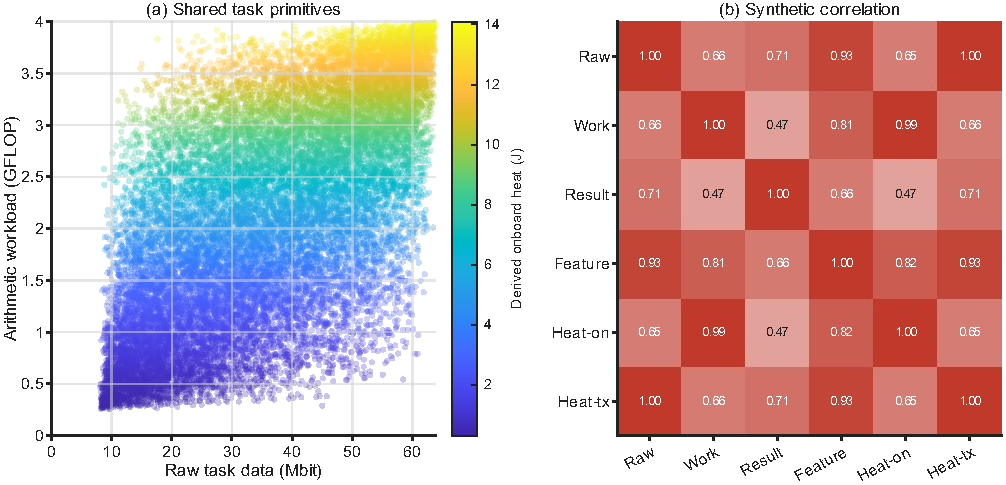
\includegraphics[width=0.98\textwidth]{figures/fig_physical_generator.pdf}
\caption{Internal-consistency audit of the synthetic generator. (a) A legibility sample of 2,000 of 20,000 tasks; color encodes heat derived from compute energy. (b) Correlations computed from all 20,000 tasks. No fitted flight distribution is implied.}
\label{fig:physical}
\end{figure}

\subsubsection{Complete stochastic generator and action-load specification}
\label{sec:complete_simulator}

To support independent reconstruction, this subsection specifies the remaining simulator functions used in the transition. Let $u_D,\epsilon_W\sim\mathcal N(0,1)$ independently, $u_W=0.68u_D+\sqrt{1-0.68^2}\epsilon_W$, and $g(u)=[1+\exp(-1.55u)]^{-1}$. Nominal raw volume and workload are
\begin{equation}
D=8+56g(u_D)\ {\rm Mbit},\qquad W=0.25+3.75g(u_W)\ {\rm GFLOP}.
\label{eq:primitive_generator}
\end{equation}
The burst interval spans indices $\lfloor T/3\rfloor$ through $\lfloor T/3\rfloor+\max(4,\lfloor T/4\rfloor)-1$ and multiplies both quantities by 1.45. With independent $U_r,U_f\sim\mathcal U(0,1)$,
\begin{align}
r&=0.01+0.04U_r,\qquad f=0.08+0.22\clip[0.65g(u_W)+0.35U_f,0,1],\notag\\
p&=0.20+0.25g(u_W),\qquad D^{res}=rD,\quad D^{feat}=fD,\quad W^{pre}=pW,\notag\\
n&=\operatorname{round}\{6+43\clip[0.60g(u_W)+0.40g(u_D),0,1]\},\qquad x_5=n^2.
\label{eq:primitive_ratios}
\end{align}
Onboard and ground rates are 4 and 80~GFLOP~s$^{-1}$, respectively. Compute power is $P_c=4+16\clip(W/4.8,0,1)^{0.70}$~W, and transmit power is 6~W. Compute and transmit heat equal 0.78 and 0.55 times their corresponding energy use, respectively. These definitions generate all 15 coordinates in Table~\ref{tab:state_dictionary}.

At reset, a single phase $\phi\sim\mathcal U(0,2\pi)$ generates the exogenous link trace
\begin{align}
\bar b_t&=\clip\left\{\kappa_b[0.62+0.23\sin(2\pi t/24+\phi)+\epsilon^b_t]-I_{link},0.12,1\right\},\notag\\
\bar\tau_t&=\clip\left\{0.55+0.35\sin(2\pi t/31+\phi/2)+\epsilon^\tau_t,0.08,1\right\},
\label{eq:link_trace}
\end{align}
where $\epsilon^b_t\sim\mathcal N(0,0.06^2)$, $\epsilon^\tau_t\sim\mathcal N(0,0.04^2)$, $\kappa_b$ is the sensitivity multiplier, and $I_{link}=0.22$ only in the link-limited regime. All tasks and link states for an episode are drawn at reset with one seeded NumPy generator.

The normalized action loads used in Eq.~\eqref{eq:transition} are stated here in action order $(\alpha_s,\alpha_g,\alpha_{s\&g})$:
\begin{align}
\widehat w&=(W,0.05W,W)/4.8,\qquad
\widehat Q=(x_1,0.20x_7,x_{10}+x_{11})/100,\notag\\
\widehat B&=(x_6,x_9,x_{15})/76.8,\notag\\
\Delta e&=\kappa_e\left(0.012+0.042\widehat w_1,
0.007+0.025\widehat B_2/b,
0.010+0.025\widehat w_3+0.018\widehat B_3/b\right),\notag\\
\Delta q&=\left(0.055\widehat w_1(1+u),
0.048\widehat B_2/b,
0.030(\widehat w_3+\widehat B_3/b)\right),\notag\\
\mu&=\left(0.030(1-u),0.035b\tau,0.032(1-0.5u)\right),\notag\\
\ell&=(0.02,0.18\widehat B_2,0.12\widehat B_3).
\label{eq:action_loads}
\end{align}
Each division by $b$ uses $\max(b,0.1)$. The utilization targets in Eq.~\eqref{eq:transition} are $(\widehat w_1,0.10\widehat B_2,0.55\widehat w_3)$. Initial resources are $(h,e,q,u)=(0.22,0.88,0.12,0.18)$. Energy-limited episodes instead use $e=0.62$, and thermal-stress episodes use $h=0.42$. Each episode terminates after exactly 64 executed actions, and the terminal Bellman multiplier is zero. Energy and the other resources remain clipped, soft-constrained accounting states. In particular, $e=0$ neither masks infeasible actions nor terminates an episode. It therefore does not represent a conserved battery state, and clipping does not retain the magnitude of an energy deficit.

\subsection{Sequential Scheduling Formulation}
\label{sec:mdp}

\subsubsection{State and transition}

The normalized 24-dimensional state is
\begin{equation}
s_t=[x_t,\eta_t,z_t],\qquad
\eta_t=[t/(T-1),\sin\phi,\cos\phi],\qquad
z_t=[h_t,e_t,q_t,u_t,b_t,\tau_t],
\end{equation}
where $x_t\in\R^{15}$ contains the task inputs defined in Table~\ref{tab:state_dictionary}. The context vector $\eta_t$ exposes absolute episode time and the reset-level link phase. Together, these variables determine the time-varying task and link distributions. The remaining task and link innovations are independent draws conditional on this context. The resource vector contains normalized heat, remaining energy, queue occupancy, compute utilization, bandwidth, and contact duration. Thus, within each fixed regime, the transition distribution is conditioned on all persistent simulator variables rather than on a hidden reset phase.

Executing action $a_t$ changes resources before the next exogenous task arrives. The implemented transition is
\begin{align}
h_{t+1}&=\clip(0.86h_t+0.17c\widehat Q_t^{(a_t)},0,1.3),\notag\\
e_{t+1}&=\clip(e_t+0.006-c\Delta e_t^{(a_t)},0,1),\notag\\
q_{t+1}&=\clip(q_t+c(\Delta q_t^{(a_t)}-\mu_t^{(a_t)}),0,1.3),\notag\\
u_{t+1}&=\clip(0.68u_t+0.32c\widehat w_t^{(a_t)},0,1.2),\notag\\
b_{t+1}&=\clip(\bar b_{t+1}-c\ell_t^{(a_t)},0.08,1),\notag\\
\tau_{t+1}&=\clip(\bar\tau_{t+1}-0.10c\widehat B_t^{(a_t)},0.05,1).
\label{eq:transition}
\end{align}
Here $\widehat Q$, $\widehat w$, and $\widehat B$ denote normalized action-specific heat, work, and data demands, respectively. The terms $\Delta e$, $\Delta q$, $\mu$, and $\ell$ are the deterministic resource-use, queue, service, and link-occupation functions defined in Eq.~\eqref{eq:action_loads}. Exogenous link variables $\bar b$ and $\bar\tau$ follow Eq.~\eqref{eq:link_trace} and are sampled before each episode. Setting $c=0$ removes action-dependent carryover, $c=0.5$ weakens it, and $c=1$ produces fully coupled dynamics.

\subsubsection{Reward and standard DQN backbone}

The reward is the negative immediate cost plus post-decision feasibility penalties:
\begin{align}
r_t={}&-c_t^{imm}-c\big[12(h_{t+1}-0.78)_+ +15(0.18-e_{t+1})_+\notag\\
&+8(q_{t+1}-0.75)_+ +10\mathbf 1_{a_t\ne\alpha_s}(0.14-\tau_t)_+\big].
\label{eq:reward}
\end{align}
The DQN uses the unmodified factual target
\begin{equation}
y_t=r_t+\gamma(1-d_t)\max_{a'}Q_{\bar\theta}(s_{t+1},a'),
\label{eq:factual}
\end{equation}
and factual loss
\begin{equation}
L_{DQN}=\mathcal H\big(Q_\theta(s_t,a_t),y_t\big),
\end{equation}
where $\mathcal H$ denotes the Huber loss. The target network both selects and evaluates the maximizing action, as required by standard DQN.

\subsection{DQN Objective Family and Full-Action Supervision}
\label{sec:method}

All six objectives share the factual Huber loss and the same implementation settings. Standard DQN members use Eq.~\eqref{eq:factual}, whereas Double DQN members use online-network action selection with target-network evaluation. Standard DQN and Double DQN learn only from factual transitions. Four model-assisted objectives additionally use a training-only auxiliary path that supplies labels for unexecuted actions. The following construction defines the shared preview interface and the centered member. The experiments also evaluate uncentered full-action Q, immediate advantage, and the corresponding Double DQN auxiliary objective.

\subsubsection{Side-effect-free full-action preview}

For every replayed factual state, the analytical transition evaluates each action $a\in\mathcal A$:
\begin{equation}
(\tilde \ell_{t,a},\tilde z'_{t,a})=F_{preview}(x_t,z_t,a).
\end{equation}
Here $\tilde \ell_{t,a}$ contains the immediate cost and post-decision feasibility penalty for action $a$. The preview does not advance time, mutate state, alter trajectories, or consume random numbers. Before action selection, it computes only the current-task cost and six post-action resources. The factual action is then executed once. After the next exogenous task $x_{t+1}$ is revealed, the replay tuple is completed. During a later replay update, all alternatives reuse this observed next task and exogenous link trace. The counterfactual next state therefore replaces only the six endogenous resource coordinates:
\begin{equation}
\tilde s'_{t,a}=[x_{t+1},\eta_{t+1},\tilde z'_{t,a}].
\end{equation}
Evaluation and deployment never call the preview interface.

\subsubsection{All-action counterfactual Bellman targets}

The simulator-exact one-step outcome yields
\begin{equation}
\tilde y_{t,a}=-\tilde \ell_{t,a}+\gamma(1-d_t)
\max_{a'}Q_{\bar\theta}(\tilde s'_{t,a},a').
\label{eq:cf_target}
\end{equation}
These targets require no multi-step rollout, and no counterfactual transition is inserted into replay. The centered full-action objective uses the targets only after the state-wise centering defined below.

\subsubsection{Centered advantage distillation}

Absolute targets in Eq.~\eqref{eq:cf_target} share a bootstrapped state-value offset. Deployment selects $\arg\max_a Q(s,a)$, so a common additive offset cannot change the action. We define predicted and target centered advantages as
\begin{align}
\widehat A_{t,a}&=Q_\theta(s_t,a)-\frac{1}{|\mathcal A|}\sum_jQ_\theta(s_t,j),\notag\\
\tilde A_{t,a}&=\tilde y_{t,a}-\frac{1}{|\mathcal A|}\sum_j\tilde y_{t,j}.
\label{eq:center}
\end{align}
The advantage and total losses are
\begin{align}
L_{adv}&=\frac{1}{|\mathcal A|}
\sum_{a\in\mathcal A}\mathcal H(\widehat A_{t,a},\tilde A_{t,a}),\notag\\
L_{CFA}&=L_{DQN}+\lambda L_{adv}.
\label{eq:cbad}
\end{align}
The factual term anchors the absolute Q scale, while $L_{adv}$ teaches all action gaps. The only added algorithmic hyperparameter is $\lambda$.

\begin{figure}[H]
\centering
\fbox{\begin{minipage}{0.93\textwidth}
\textbf{Algorithm 1: DQN training with centered full-action supervision}
\begin{enumerate}[leftmargin=1.6em,itemsep=2pt,topsep=4pt]
\item Initialize uniform replay $\mathcal D$, online $Q_\theta$, and target $Q_{\bar\theta}\leftarrow Q_\theta$.
\item At each real step, observe $s_t$ and preview current-task outcomes $(\tilde \ell_{t,a},\tilde z'_{t,a})$ for all actions without side effects.
\item Select $a_t$ by the shared epsilon-greedy schedule and execute it once. After $x_{t+1}$ is revealed, store the factual tuple plus the previously computed previews.
\item When an update is due, sample one uniform mini-batch, compute the factual loss, compute Eqs.~\eqref{eq:cf_target} and \eqref{eq:center}, and update $\theta$ using Eq.~\eqref{eq:cbad}.
\item Synchronize $Q_{\bar\theta}$ at the shared fixed interval.
\end{enumerate}
\end{minipage}}
\par\smallskip
\caption*{Training previews are never used for evaluation or deployment.}
\label{alg:cbad}
\end{figure}

\subsection{Experimental Design and Settings}
\label{sec:experiments}

\subsubsection{Design principles}

\begin{revisedblock}
The six objectives were selected as a compact matched family spanning three design questions on one DQN backbone: factual-only versus full-action supervision, absolute versus centered or immediate targets, and standard versus Double-DQN target evaluation. The design separates primary family-level inference from secondary within-family analyses. The primary analysis compares all six DQN objectives with MPC-4 across five fully coupled regimes. This design yields \DQNvsMPCContrastCount{} objective--regime contrasts under shared seed blocks and traces. Secondary analyses describe how auxiliary supervision and Double DQN target evaluation coincide with performance changes within the family. The standard-DQN versus centered full-action contrast describes the addition of that complete auxiliary objective to an otherwise unchanged factual DQN backbone. Full-action Q and immediate advantage use the same three modeled outcomes per state, matching the type and number of model outputs. However, these comparisons do not isolate centering or Bellman bootstrapping because target scales differ and auxiliary weights were not tuned separately. The Double-DQN contrast is likewise a fixed-coefficient description under decoupled action selection and target evaluation~\cite{vanhasselt2016double}. The $c\in\{0,0.5,1\}$ regimes and $H\in\{1,2,4,6\}$ planning horizons bound the comparison across coupling and planning depth.
\end{revisedblock}

Standard DQN and its centered full-action variant differ only in the auxiliary objective. They share the same input, network, replay, exploration, optimizer, update cadence, target synchronization, and gradient clipping. The full-action Q control applies the same auxiliary weight directly to the three uncentered Bellman targets. The immediate-advantage control centers the negative analytical one-step costs but omits their bootstrapped future values. Both Double DQN variants use online-network action selection with target-network evaluation in factual and auxiliary Bellman targets. Dueling networks, prioritized replay, multi-step returns, noisy networks, and distributional value learning remain outside the comparison.

We fixed the auxiliary weight before running experiments with the internally consistent simulator. A preceding calibration with model seeds 700--703 compared $\lambda\in\{0.1,0.3,1,3\}$. The rule selected $\lambda=0.3$ by maximizing the worst relative improvement of the centered full-action variant across five coupled regimes. Ties favored the smaller weight. This rule was specific to the centered objective. The uncentered full-action, immediate-advantage, and Double DQN auxiliary variants inherited $\lambda=0.3$ without method-specific calibration. Because the auxiliary losses differ in scale and error structure, these are fixed-coefficient implementation comparisons. They do not factorially isolate centering or bootstrapping. The calibration used an earlier simulator version and therefore serves as a prior specification rather than evidence from the current generator. Confirmatory and component analyses use seeds 800--819 without post hoc removal, replacement, or selection. Every learned policy was trained only on the nominal $c=1$ distribution.

\subsubsection{Training configuration}

Each network has 24 inputs, hidden widths of 128--128--64, rectified linear unit (ReLU) activations, and three outputs. Every model receives 600 episodes of 64 tasks, totaling 38,400 real interactions. Fixed settings are $\gamma=0.97$, a learning rate of $3\times10^{-4}$, a batch size of 128, a replay capacity of 100,000, and a gradient-norm limit of 10. Training begins after 128 transitions and performs one update every four interactions. The checkpoint field \texttt{target\_interval=250} is evaluated only on update calls. Because updates occur at interaction counts divisible by four, synchronization occurs every 500 real interactions, equivalent to 125 optimizer updates. Epsilon decreases linearly from 1 to 0.05 over 13,440 interactions.

The contextual bandit uses the same network, optimizer, exploration schedule, and interaction budget, with $\gamma=0$. It therefore learns the modeled one-step reward without a long-horizon Bellman term. Uniform replay stores only one-step factual transitions, with preview outputs attached as auxiliary training data. Standard DQN and Double DQN do not use analytical labels for alternative actions. The four auxiliary variants evaluate all three modeled action outcomes at every real interaction. The checkpoint manifest records these counts, optimizer updates, and wall time for every trained model.

All reported experiments use the internally consistent synthetic generator described above. Link bandwidth and contact duration follow bounded, noisy periodic traces generated at reset. Burst and thermal-stress episodes multiply raw data and workload by 1.45 during one contiguous interval. All dependent heat, energy, latency, and transmission quantities are then recomputed from those primitives. An earlier independently sampled generator is retained only as a historical reproducibility mode and is not used for the reported results.

\subsubsection{Seven evaluation regimes}

The seven regimes comprise two composite coupling-boundary conditions and five fully coupled operating conditions:

\begin{enumerate}[leftmargin=1.6em]
    \item \textbf{Static ($c=0$):} removes action-dependent state transitions and scales delayed feasibility penalties to zero.
    \item \textbf{Reduced coupling ($c=0.5$):} halves action-dependent resource effects and the delayed feasibility-penalty scale.
    \item \textbf{Nominal ($c=1$):} matches the fully coupled training distribution.
    \item \textbf{Burst:} increases contiguous compute and thermal demand.
    \item \textbf{Link-limited:} reduces the available bandwidth trace by 0.22 before clipping.
    \item \textbf{Energy-limited:} lowers initial energy from 0.88 to 0.62.
    \item \textbf{Thermal-stress:} raises initial heat from 0.22 to 0.42 and includes the burst interval.
\end{enumerate}

The first two regimes are composite interventions because $c$ scales both the transition in Eq.~\eqref{eq:transition} and the delayed-penalty term in Eq.~\eqref{eq:reward}. They therefore do not isolate action-dependent carryover from reward rescaling. The remaining five regimes retain $c=1$. Models trained at $c=1$ are transferred to the two boundary conditions without retraining. These rows measure behavior under a joint objective-and-dynamics shift rather than the best policy attainable at lower coupling.

\subsubsection{Planning comparator, outcomes, and inference}

\begin{revisedblock}
The deployment comparison includes immediate-cost argmin, a contextual bandit, a prespecified resource-threshold heuristic, standard DQN, the centered full-action family member, an eight-step greedy rollout, and an exact $H$-step receding-horizon planner. MPC-4 is the prespecified primary planning comparator because four steps provide nontrivial look-ahead while retaining transparent exhaustive enumeration at every decision. The planning-depth study shows the trade-off rather than treating $H=4$ as globally optimal: $H=1$ is myopic, while enumeration grows as $3^H$. The greedy rollout enumerates each first action and then selects the lowest predicted one-step cost for seven subsequent steps, executes only the first action, and replans. The threshold heuristic first checks whether $h>0.72$ or $e<0.24$. If this condition holds and both $b>0.28$ and $\tau>0.18$, it selects ground processing; otherwise, it selects collaborative processing. When neither heat nor energy triggers the rule, it selects onboard processing if $b<0.22$ or $\tau<0.14$. If this bandwidth or contact condition is also absent, it selects collaborative processing when $q>0.70$ and immediate-cost argmin otherwise. These thresholds were specified manually and were not fitted to the evaluation traces. Fixed onboard and fixed ground policies always select $\alpha_s$ and $\alpha_g$, respectively. At each decision, the planner enumerates all $3^H$ action sequences over the next $H$ known tasks and link states. It minimizes discounted modeled cost with $\gamma=0.97$, executes only the first action, and replans. The primary table reports $H=4$. A separate nominal analysis evaluates $H\in\{1,2,4,6\}$ on 400 unique held-out traces and reports wall-clock time per decision. Each planner is exact only for its stated perfect-forecast objective, not for the 64-step global problem. Both MPC and greedy rollout receive perfect next-task and link-state previews; learned policies receive only the current state, so the comparison includes an explicit information asymmetry.
\end{revisedblock}

The primary outcome is the undiscounted episode total cost
\begin{equation}
C_{\mathrm{episode}}=\sum_{t=0}^{T-1}\left(c^{\mathrm{imm}}_t+p_t\right)=-\sum_{t=0}^{T-1}r_t,
\label{eq:episode_cost}
\end{equation}
\begin{revisedblock}
where $p_t$ is the complete nonnegative penalty inside the square brackets in Eq.~\eqref{eq:reward}, including its multiplier $c$. Every executed step, including the terminal step, contributes once. DQN and the finite-horizon planner optimize discounted targets, whereas Eq.~\eqref{eq:episode_cost} reports accumulated operational cost without discounting. The nominal sensitivity experiment varies the shared planning and learning discount over $\gamma\in\{0.90,0.95,0.97,0.99\}$. Secondary outcomes are immediate cost, delayed penalty, energy use, modeled latency, transmitted data, threshold-exposure steps, planner wall-clock time, maximum heat, and minimum remaining energy.
\end{revisedblock}

The independent inferential unit is the model-seed block. For learned--learned comparisons, the same seed initializes network weights and controls task seeds, exploration draws, and replay-index sampling. Trajectories may diverge after different greedy actions, but the matched seed remains the randomization block. Each seed is evaluated on the same 20 held-out traces, which are averaged within seed. This procedure gives $n=20$ blocks per learned method. For the central DQN-family--MPC-4 claim, each raw row is matched by regime, model-seed trace namespace, and trace seed. Trace-level differences are then averaged within seed. MPC-4 is deterministic conditional on a trace; its model-seed field therefore indexes a matched trace namespace rather than a trained planner replicate.

All paired bootstrap analyses use 10,000 resamples with seed 20260829. Individual two-sided 95\% intervals are percentile intervals, and exact two-sided paired sign tests assess directional consistency. For the \DQNvsMPCContrastCount{} DQN-objective--regime contrasts against MPC-4, one joint bootstrap resamples the same 20 seed blocks across all contrasts. This procedure preserves correlation among the contrasts. Sign-test values are Holm-adjusted across all cells. We also report the largest, least-favorable mean difference within each regime and across the complete contrast set. A simultaneous one-sided 95\% upper bound adds a joint critical value to every observed cell mean. The critical value is the 95th percentile of the largest centered bootstrap deviation across the relevant cells. An upper bound below zero supports the joint statement that every mean difference is negative. For within-family contrasts, Holm adjustment is applied across the five fully coupled regimes separately for each prespecified contrast. The eight parameter profiles form a separate family, and each preview-scale contrast forms its own five-regime family. A directional cell is labeled supported only if its mean favors the first-named method, its paired interval excludes zero, and its family-adjusted sign-test value is below 0.05. We report seed-level differences and leave-one-seed-out ranges for the prespecified centered full-action versus standard DQN contrast. Its conservative sensitivity analysis resamples the two sets of 20 seed means independently and ignores matching. Test traces and bootstrap draws are never treated as independent model replicates.

\subsubsection{Prespecified sensitivity and training diagnostics}

Without retraining or model selection, we repeated the nominal evaluation under eight profiles. They covered the reference configuration, compute demand $\pm20\%$, raw data volume $\pm20\%$, energy use $+20\%$, heat load $+20\%$, and link capacity $-20\%$. Each profile retained the same 20 models and held-out trace namespace as the primary experiment. Holm adjustment covered all eight profiles. Training logs record every episode for all 20 seeds. Curves report a causal 25-episode moving mean and the seed-level mean $\pm$ standard deviation (SD) for total cost, energy use, latency, and delayed penalty. These diagnostics describe optimization trajectories; confirmatory claims remain based on held-out traces.

\begin{revisedblock}
\subsubsection{Second-round sensitivity and matched decision-time experiments}
\label{sec:revision_experiments}

To test value-horizon sensitivity, we retrained all six objectives at $\gamma\in\{0.90,0.95,0.97,0.99\}$ on the nominal generator. Each cell used 20 model seeds, 600 episodes of 64 interactions, and the same 20 held-out traces per seed. The $\gamma=0.97$ row is the locked reference. The same paired seed blocks and 10,000-resample bootstrap were retained, while the 18 alternative-gamma contrasts formed a separate Holm family. MPC-4 was tested at the corresponding four discount factors on the same traces. Training-length sensitivity used $\gamma=0.97$ and 900 episodes with checkpoints at episodes 300, 600, and 900. The epsilon schedule remained fixed at 13,440 interactions so that the comparison changes training exposure rather than exploration decay. All six logged objectives are shown in the learning-curve figure, using the same causal smoothing and across-seed variation display.

For deployment cost and latency, we evaluated the six DQN policies, MPC-4, and the eight-step greedy rollout on shared nominal states. All decision times were measured on one CPU thread with batch size one after warm-up; three timed repetitions were summarized by mean, median, and 95th percentile. The greedy baseline uses the same perfect forecast as MPC, while DQN timing uses only the current state. New gamma, training-length, and baseline-cost comparisons use separate paired bootstrap and Holm families and are not mixed with the original 30-cell family comparison. Runtime summaries are descriptive measurements of the tested software and hardware. The experiment code writes immutable manifests, raw seed-level results, and validation summaries under \texttt{results/revision\_round2/}.
\end{revisedblock}

\subsubsection{Preview-model misspecification test}

The main experiment assumes that the analytical preview matches the simulator transition. To test this dependence, we trained two additional centered full-action model sets without changing the factual environment or deployment evaluation. One set scaled preview one-step costs and action-induced resource changes by 0.85, while the other used 1.15. The preview cost comprised the immediate cost and modeled penalty. Resource predictions were clipped to the same physical bounds after scaling around the current resource state. Each condition used the same 20 seeds, training budget, network, replay, and held-out trace namespace as the main experiment. These symmetric stress-test scales were fixed in advance and were not used for model selection.

\subsubsection{Reproducible result entry point}

The core result entry point is \texttt{python -m dqn\_family\_satellite\_ground.\allowbreak reviewer\_experiments all \allowbreak --seeds 800-819 \allowbreak --resume}. Component and Double DQN comparisons use \texttt{python -m dqn\_family\_satellite\_ground.\allowbreak extended\_revision \allowbreak --seeds 800-819 \allowbreak --stage all \allowbreak --resume}. The first command trains or loads 60 primary learned-policy checkpoints and 40 preview-error checkpoints. The second reuses the primary DQN checkpoints and trains 80 component and Double DQN checkpoints. It then evaluates six DQN objectives, performs the independent-seed bootstrap, and evaluates four planning depths on 400 unique traces.

The command \texttt{python -m dqn\_family\_satellite\_ground.\allowbreak extended\_reporting} recomputes the \DQNvsMPCContrastCount{} paired DQN--MPC-4 contrasts, joint maximum statistics, LaTeX tables, and artifact hashes from locked raw comma-separated value (CSV) files. The command \texttt{python -m dqn\_family\_satellite\_ground.\allowbreak transition\_audit} writes a fixed-seed, all-action example. In this example, preview and executed costs and all six resources agree coordinate by coordinate. Unit tests repeat this comparison at both clipping boundaries and on the terminal step. They also verify that time and link phase occupy the three added state coordinates.

Experiments used Python 3.13.9, NumPy 2.4.1, pandas 3.0.3, and PyTorch 2.8.0 with CUDA 12.9. Hardware comprised an NVIDIA GeForce RTX 5070 Ti running Windows 11. Planning wall time was measured on a 12th Gen Intel Core i9-12900K with 24 logical processors after one untimed warm-up episode. Reported values are means over all timed decisions. Machine-readable metadata record the 24-dimensional state definition, resolved variants, seeds, budgets, randomization blocks, model-information counts, result files, and runtime environment. Table and figure scripts consume these files directly.

\section{Results}
\label{sec:results}

\subsection{Direct paired inference supports a DQN-family advantage under full coupling}

\revised{We first tested the prespecified family-level claim against MPC-4. Among the original non-DQN comparator set, MPC-4 had the lowest mean in every fully coupled regime. All \DQNvsMPCContrastCount{} paired objective--regime comparisons produced lower mean costs for DQN, and every individual 95\% bootstrap interval excluded zero.}

\begin{table}[H]
\centering
\caption{Episode total cost under the internally consistent synthetic generator. For learned policies, standard deviation (SD) is calculated across 20 independently trained model-seed blocks after within-seed trace averaging. For deterministic non-learned policies, SD is calculated across 20 disjoint trace namespaces and does not represent training variability. These quantities describe different sources of variation and are not directly comparable as inferential uncertainty. All learned policies were trained only at nominal $c=1$; static and reduced-coupling rows are transfers without retraining. MPC-4 is exact only for its stated four-step perfect-forecast objective. Lower values are better.}
\label{tab:main}
\resizebox{\textwidth}{!}{\begin{tabular}{lrrrrrr}
\toprule
Regime & Argmin & MPC-4 & Bandit & Threshold & DQN & Centered FA \\
\midrule
Static ($c=0$) & 24.55 $\pm$ 0.21 & 24.55 $\pm$ 0.21 & 24.78 $\pm$ 0.33 & 24.74 $\pm$ 0.25 & 26.85 $\pm$ 0.99 & 26.66 $\pm$ 0.64 \\
Reduced ($c=0.5$) & 26.65 $\pm$ 0.63 & 25.70 $\pm$ 0.26 & 26.39 $\pm$ 1.05 & 26.43 $\pm$ 0.38 & 27.81 $\pm$ 0.68 & 27.61 $\pm$ 0.56 \\
Nominal & 193.42 $\pm$ 8.33 & 90.83 $\pm$ 1.71 & 101.00 $\pm$ 4.94 & 188.08 $\pm$ 6.41 & 78.33 $\pm$ 1.88 & 77.66 $\pm$ 1.84 \\
Burst & 241.20 $\pm$ 6.84 & 108.35 $\pm$ 1.99 & 136.55 $\pm$ 11.20 & 238.74 $\pm$ 6.56 & 97.36 $\pm$ 2.01 & 96.88 $\pm$ 1.94 \\
Link-limited & 272.02 $\pm$ 7.98 & 115.73 $\pm$ 1.92 & 139.75 $\pm$ 7.36 & 227.25 $\pm$ 8.36 & 102.26 $\pm$ 1.75 & 101.80 $\pm$ 1.80 \\
Energy-limited & 225.31 $\pm$ 7.73 & 126.00 $\pm$ 1.58 & 133.26 $\pm$ 4.20 & 246.46 $\pm$ 6.45 & 119.67 $\pm$ 2.14 & 119.00 $\pm$ 1.65 \\
Thermal-stress & 247.58 $\pm$ 6.25 & 109.20 $\pm$ 2.01 & 137.74 $\pm$ 10.79 & 241.80 $\pm$ 6.26 & 97.55 $\pm$ 2.03 & 97.10 $\pm$ 1.93 \\
\bottomrule
\end{tabular}}
\end{table}

\begin{figure}[H]
\centering
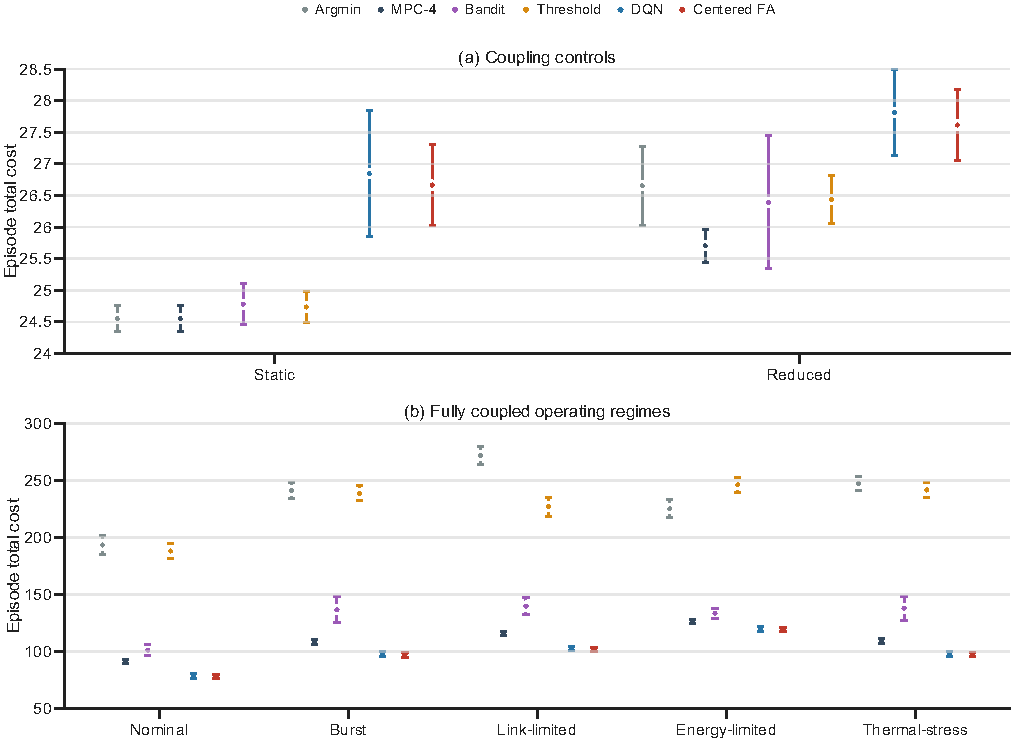
\includegraphics[width=0.98\textwidth]{figures/fig_reviewer_primary.pdf}
\caption{Performance across seven regimes under internally consistent synthetic task generation. For learned policies, error bars show SD across 20 model-seed blocks after within-seed trace averaging. Deterministic comparators show variation across trace namespaces, so their error bars are descriptive and not inferentially interchangeable with those of learned methods. All learned models were trained at nominal $c=1$; the $c<1$ rows are transfers without retraining. The ordinate differs among panels, so panel heights should not be compared directly.}
\label{fig:seven}
\end{figure}

\begin{table}[H]
\centering
\caption{Direct joint inference for the DQN family relative to MPC-4. Differences are DQN minus MPC-4, so negative values favor DQN. Within each regime, the table reports the largest, least-favorable mean among six DQN-objective contrasts; the final row takes the maximum across all 30 objective--regime cells. Intervals are percentile intervals for the corresponding maximum from 10,000 joint bootstrap resamples. Simultaneous one-sided 95\% upper bounds use the maximum centered bootstrap deviation. The independent unit is the model-seed block ($n=20$), after averaging 20 shared held-out traces within each block.}
\label{tab:dqn_vs_mpc_family}
\resizebox{\textwidth}{!}{\begin{tabular}{llrrr}
\toprule
Scope & Least-favorable DQN objective & Maximum $\Delta$ & 95\% interval for maximum & Simultaneous 95\% upper bound \\
\midrule
Nominal & Double DQN & -12.43 & [-12.92, -11.81] & -11.82 \\
Burst & Double DQN & -10.74 & [-11.26, -10.13] & -10.17 \\
Link-limited & Double DQN & -13.15 & [-13.65, -12.58] & -12.62 \\
Energy-limited & Double DQN & -5.92 & [-6.66, -4.94] & -5.04 \\
Thermal-stress & Double DQN & -11.40 & [-11.94, -10.77] & -10.84 \\
All five regimes & Double DQN (Energy-limited) & -5.92 & [-6.66, -4.94] & -5.03 \\
\bottomrule
\end{tabular}}
\end{table}

The joint seed-block analysis supported the same conclusion after multiplicity correction across all \DQNvsMPCContrastCount{} cells. Every seed block favored DQN, and the largest Holm-adjusted sign-test value was \DQNvsMPCHolmPMax. The least-favorable cell was Double DQN under energy limitation. Its mean difference was \DQNvsMPCGlobalWorstDifference{}, with a simultaneous 95\% upper bound of \DQNvsMPCGlobalUpperBound{} (Table~\ref{tab:dqn_vs_mpc_family}; Fig.~\ref{fig:graphical}). Nominal DQN-family means spanned \DQNFamilyNominalMinCost--\DQNFamilyNominalMaxCost, compared with \MPCNominalCost{} for MPC-4. Together, these analyses support a DQN-family advantage as the central benchmark finding.

\subsection{Target design produces smaller, scenario-dependent differences within the DQN family}

\begin{table}[H]
\centering
\caption{Episode total cost across six DQN objectives in the five fully coupled regimes. Values are mean $\pm$ SD across 20 independently trained model-seed blocks after within-seed averaging of 20 shared held-out traces. Lower values are better, and the leading objective varies across regimes.}
\label{tab:dqn_family}
\resizebox{\textwidth}{!}{\begin{tabular}{lrrrrr}
\toprule
Training objective & Nominal & Burst & Link-limited & Energy-limited & Thermal-stress \\
\midrule
Standard DQN & 78.33 $\pm$ 1.88 & 97.36 $\pm$ 2.01 & 102.26 $\pm$ 1.75 & 119.67 $\pm$ 2.14 & 97.55 $\pm$ 2.03 \\
Full-action Q auxiliary & 78.14 $\pm$ 2.23 & 97.21 $\pm$ 2.25 & 102.17 $\pm$ 2.09 & 119.78 $\pm$ 2.38 & 97.41 $\pm$ 2.25 \\
Immediate advantage auxiliary & 77.84 $\pm$ 1.82 & 97.22 $\pm$ 2.05 & 101.95 $\pm$ 1.88 & 119.17 $\pm$ 2.12 & 97.40 $\pm$ 2.04 \\
Centered full-action & 77.66 $\pm$ 1.84 & 96.88 $\pm$ 1.94 & 101.80 $\pm$ 1.80 & 119.00 $\pm$ 1.65 & 97.10 $\pm$ 1.93 \\
Double DQN & 78.40 $\pm$ 1.98 & 97.61 $\pm$ 2.15 & 102.59 $\pm$ 2.08 & 120.08 $\pm$ 2.41 & 97.80 $\pm$ 2.12 \\
Double + centered full-action & 77.73 $\pm$ 1.99 & 96.90 $\pm$ 2.02 & 101.91 $\pm$ 1.88 & 119.07 $\pm$ 1.77 & 97.13 $\pm$ 2.01 \\
\bottomrule
\end{tabular}}
\end{table}

\begin{figure}[H]
\centering
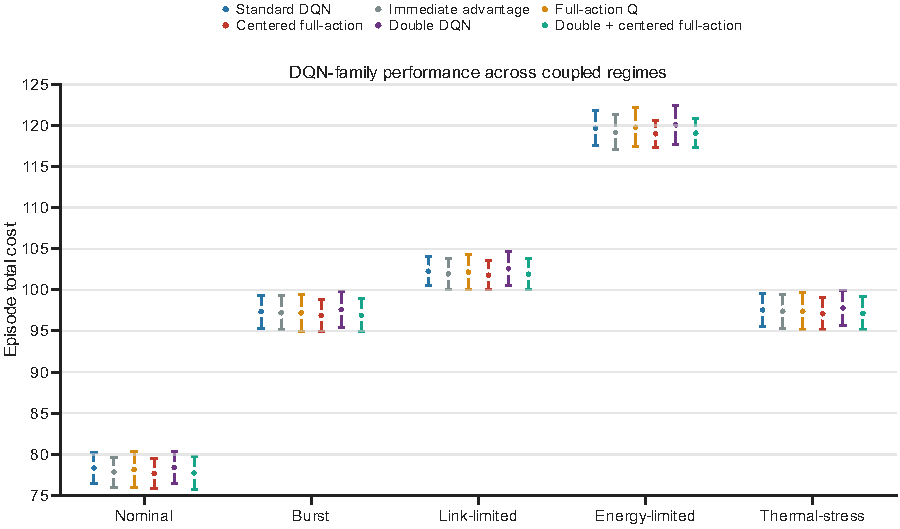
\includegraphics[width=0.98\textwidth]{figures/fig_dqn_family.pdf}
\caption{DQN-family performance across fully coupled regimes. Points show model-seed means and error bars show $\pm$1 SD across 20 independently trained model seeds. The figure shows overlapping distributions and scenario-dependent ordering across objectives.}
\label{fig:dqn_family}
\end{figure}

\begin{table}[H]
\centering
\caption{Nominal fixed-coefficient component and backbone comparisons. All models use 20 prespecified model-seed blocks, identical real-interaction budgets, and the same held-out traces. Full-action Q and immediate advantage receive the same three modeled action outcomes as the centered full-action variant. The shared $\lambda=0.3$ was calibrated for the centered objective and not tuned separately for the other auxiliary losses, so these rows do not isolate centering or bootstrapping. Holm adjustment covers the five fully coupled regimes separately for each displayed contrast. ``Supported'' requires a favorable mean, a paired interval below zero, and Holm $p<0.05$.}
\label{tab:extended_ablation}
\resizebox{\textwidth}{!}{\begin{tabular}{lrrrrr}
\toprule
Training objective & Mean cost $\pm$ SD & Matched reference & Paired difference [95\% interval] & Holm $p$ & Supported \\
\midrule
Standard DQN & 78.33 $\pm$ 1.88 & -- & -- & -- & -- \\
Full-action Q auxiliary & 78.14 $\pm$ 2.23 & Standard DQN & -0.19 [-0.56, 0.28] & 0.05909 & No \\
Immediate advantage auxiliary & 77.84 $\pm$ 1.82 & Standard DQN & -0.49 [-0.90, -0.12] & 1 & No \\
Centered full-action & 77.66 $\pm$ 1.84 & Standard DQN & -0.67 [-0.99, -0.39] & 0.01288 & Yes \\
Double DQN & 78.40 $\pm$ 1.98 & -- & -- & -- & -- \\
Double + centered full-action & 77.73 $\pm$ 1.99 & Double DQN & -0.67 [-1.18, -0.24] & 0.03545 & Yes \\
\bottomrule
\end{tabular}}
\end{table}

\begin{table}[H]
\centering
\caption{Paired inference for centered full-action minus standard DQN across the five fully coupled regimes. Negative differences favor centered full-action supervision. Each comparison uses 20 model-seed blocks after averaging 20 shared held-out traces. Holm adjustment covers the five prespecified regimes, and LOO denotes the leave-one-seed-out mean range.}
\label{tab:primary_inference}
\resizebox{\textwidth}{!}{\begin{tabular}{lrrrrr}
\toprule
Regime & Mean difference & 95\% interval & Negative seeds & Holm $p$ & LOO range \\
\midrule
Nominal & -0.67 & [-0.99, -0.39] & 17/20 & 0.01288 & [-0.71, -0.55] \\
Burst & -0.48 & [-0.73, -0.28] & 17/20 & 0.01288 & [-0.51, -0.37] \\
Link-limited & -0.46 & [-0.77, -0.17] & 15/20 & 0.08278 & [-0.52, -0.38] \\
Energy-limited & -0.68 & [-1.17, -0.21] & 16/20 & 0.03545 & [-0.79, -0.51] \\
Thermal-stress & -0.45 & [-0.75, -0.22] & 15/20 & 0.08278 & [-0.48, -0.33] \\
\bottomrule
\end{tabular}}
\end{table}

\begin{table}[H]
\centering
\caption{Training information and computation accounting. Wall time is mean $\pm$ SD across 20 models. ``Modeled action outcomes'' counts analytical action evaluations used by the learning objective. Information and computational budgets additionally reflect these modeled action outcomes.}
\label{tab:training_accounting}
\resizebox{0.92\textwidth}{!}{\begin{tabular}{lrrrrr}
\toprule
Training objective & Wall time per model (s) & Real interactions & Updates & Modeled action outcomes & Models \\
\midrule
Standard DQN & 37.4 $\pm$ 10.4 & 38,400 & 9,569 & 0 & 20 \\
Full-action Q auxiliary & 46.0 $\pm$ 1.4 & 38,400 & 9,569 & 115,200 & 20 \\
Immediate advantage auxiliary & 42.9 $\pm$ 1.1 & 38,400 & 9,569 & 115,200 & 20 \\
Centered full-action & 49.0 $\pm$ 3.1 & 38,400 & 9,569 & 115,200 & 20 \\
Double DQN & 36.0 $\pm$ 1.6 & 38,400 & 9,569 & 0 & 20 \\
Double + centered full-action & 53.2 $\pm$ 3.9 & 38,400 & 9,569 & 115,200 & 20 \\
\bottomrule
\end{tabular}}
\end{table}

Across the five fully coupled regimes, the six objectives occupied a narrow performance band (Table~\ref{tab:dqn_family}; Fig.~\ref{fig:dqn_family}). Nominal means ranged from \DQNFamilyNominalMinCost{} to \DQNFamilyNominalMaxCost. The leading objective varied by regime, and the gap to MPC-4 exceeded the differences among target designs.

Centered full-action produced favorable mean differences against standard DQN in all five regimes and met the complete support rule in \PrimarySupportedCount{} (Table~\ref{tab:primary_inference}). The remaining component and Double DQN contrasts produced smaller, scenario-dependent changes in ordering (Table~\ref{tab:extended_ablation}). All objectives used the same real-interaction budget, whereas the auxiliary objectives additionally consumed modeled action outcomes (Table~\ref{tab:training_accounting}).

\subsection{The DQN family remains below deeper exact planning in nominal cost}

\begin{table}[H]
\centering
\caption{\revised{Nominal receding-horizon planning over 400 unique held-out traces. Each planner has perfect knowledge of the next $H$ tasks and exogenous link states and exactly enumerates $3^H$ sequences before every action. Runtime was measured on the same workstation and includes only planner action selection after environment construction. The separate matched latency comparison, including DQN inference, is reported in Table~\ref{tab:revision_runtime}.}}
\label{tab:planner_depth}
\resizebox{0.85\textwidth}{!}{\begin{tabular}{rrrrr}
\toprule
Planning horizon & Enumerated sequences & Mean cost & Time per decision (ms) & Held-out traces \\
\midrule
1 & 3 & 99.33 & 0.13 & 400 \\
2 & 9 & 92.80 & 0.50 & 400 \\
4 & 81 & 90.83 & 4.82 & 400 \\
6 & 729 & 89.35 & 42.50 & 400 \\
\bottomrule
\end{tabular}}
\end{table}

Increasing planning depth reduced nominal mean cost from \PlannerCostHOne{} at $H=1$ to \PlannerCostHSix{} at $H=6$. Over the same range, mean decision time increased from \PlannerTimeHOne{} to \PlannerTimeHSix{} ms. At $H=6$, the nominal MPC cost remained above the DQN-family range of \DQNFamilyNominalMinCost--\DQNFamilyNominalMaxCost. Thus, within the tested horizons, deeper exact planning did not close the nominal cost gap.

\begin{table}[H]
\centering
\caption{Engineering outcome decomposition for standard DQN relative to MPC-4. Standard DQN is shown as a conventional representative of the six-objective family. Delta columns report standard DQN minus MPC-4; negative values denote lower use or cost. Low-energy steps are soft-threshold exposure counts for decisions with remaining energy below 0.18.}
\label{tab:engineering}
\footnotesize
\setlength{\tabcolsep}{2.5pt}
\begin{tabular}{lrrrrr}
\toprule
Regime & $\Delta$ immediate & $\Delta$ penalty & $\Delta$ energy & $\Delta$ latency (s) & $\Delta$ data (Mbit) \\
\midrule
Nominal & 0.76 & -13.26 & -0.104 & -1.04 & -543.9 \\
Burst & 0.42 & -11.40 & -0.098 & -0.92 & -489.8 \\
Link-limited & -0.57 & -12.91 & -0.130 & -1.46 & -388.1 \\
Energy-limited & 1.36 & -7.68 & -0.102 & -0.93 & -601.5 \\
Thermal-stress & 0.32 & -11.97 & -0.100 & -0.97 & -482.5 \\
\bottomrule
\end{tabular}
\par\medskip
\begin{tabular}{lrrr}
\toprule
Regime & Low-energy steps DQN/MPC-4 & Min. energy DQN/MPC-4 & Max. heat DQN/MPC-4 \\
\midrule
Nominal & 23.6/28.5 & 0.00/0.00 & 0.192/0.190 \\
Burst & 28.8/32.3 & 0.00/0.00 & 0.192/0.190 \\
Link-limited & 30.2/35.0 & 0.00/0.00 & 0.193/0.191 \\
Energy-limited & 38.8/41.8 & 0.00/0.00 & 0.193/0.190 \\
Thermal-stress & 28.8/32.4 & 0.00/0.00 & 0.364/0.362 \\
\bottomrule
\end{tabular}
\end{table}

Table~\ref{tab:engineering} provides a representative decomposition of the gap between standard DQN and MPC-4. Relative to MPC-4, standard DQN reduced delayed penalties in every fully coupled regime while changing immediate cost by only $-0.57$ to $1.36$. It also used less modeled energy, had lower modeled latency, and transmitted less data. Both methods reached zero in the clipped energy state, whereas standard DQN produced slightly higher maximum heat. This resource-use decomposition applies only to standard DQN.

\begin{revisedblock}
\subsection{DQN-family training diagnostics show empirical stabilization}

\begin{figure}[H]
\centering
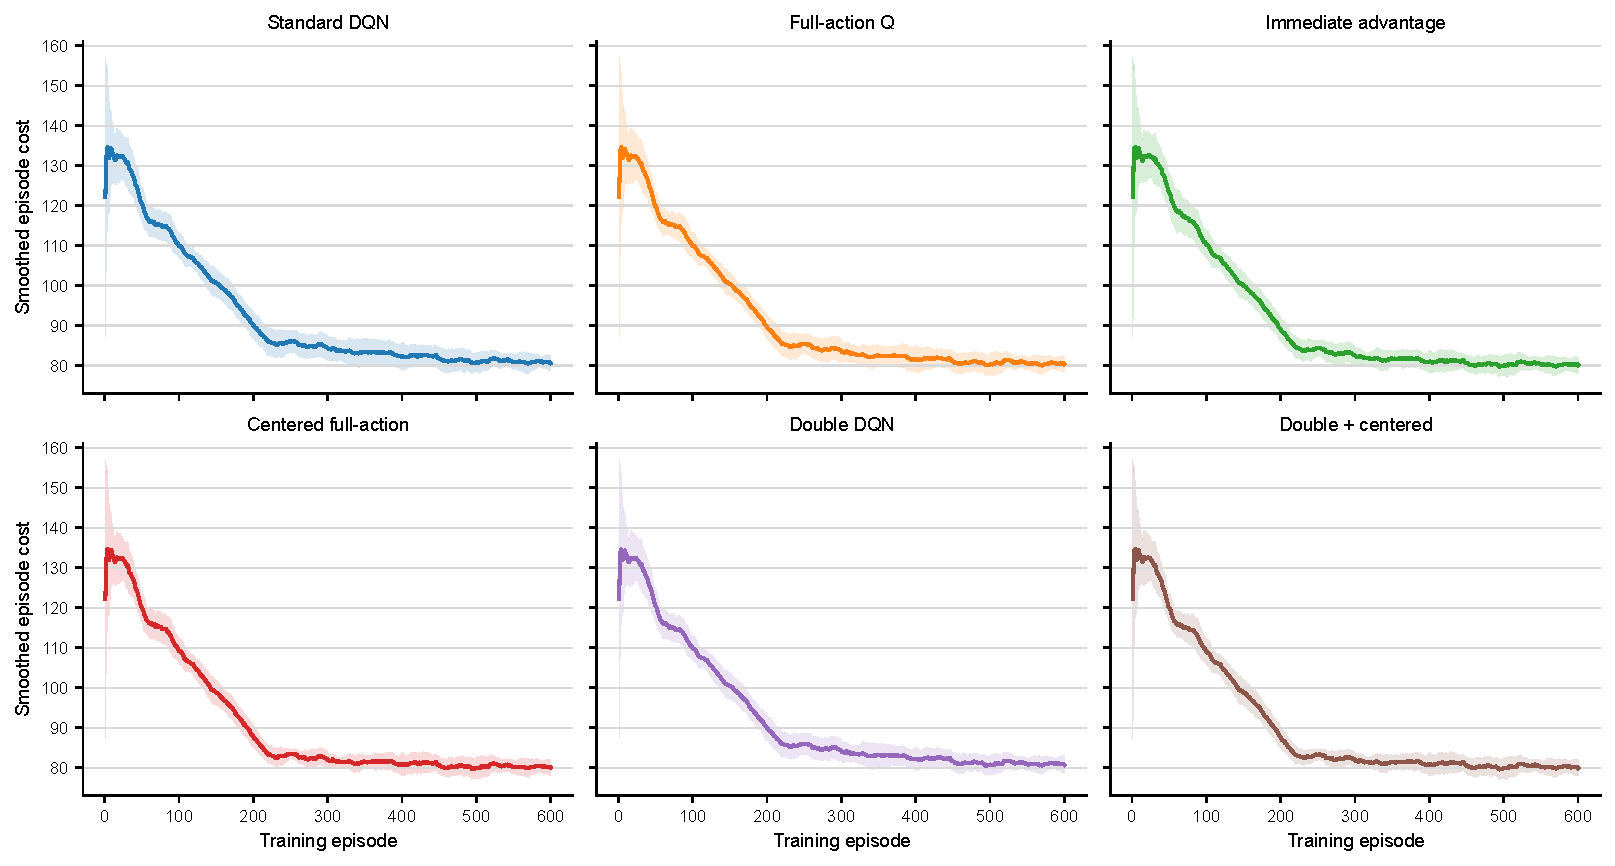
\includegraphics[width=0.98\textwidth]{figures/fig_revision_learning_curves.pdf}
\caption{Training diagnostics for all six DQN objectives. Lines are means across 20 model seeds after a causal 25-episode moving average; shaded regions are $\pm$1 SD. Curves describe optimization on the training distribution and are not treated as independent test observations.}
\label{fig:training}
\end{figure}

The late-episode trajectories in Fig.~\ref{fig:training} provide a common convergence diagnostic for all six objectives. Held-out checkpoint evaluations below distinguish stabilization of the logged training cost from generalization to the nominal test traces.

\subsection{Discount-factor and training-length sensitivity}

The second-round nominal experiment evaluated all six objectives at $\gamma=0.90$, $0.95$, $0.97$, and $0.99$ using the same seed blocks and held-out traces. Figure~\ref{fig:revision_sensitivity}a reports seed-block means and 95\% bootstrap intervals, with the locked $\gamma=0.97$ setting as the reference. The 18 alternative-gamma contrasts form a separate Holm family from the primary DQN--MPC comparison. MPC-4 was evaluated at each corresponding discount on the same traces.

At $\gamma=0.95$, none of the six contrasts with $\gamma=0.97$ was supported after Holm correction. Reducing $\gamma$ to 0.90 increased mean cost for every objective by 2.63--4.57, with all adjusted sign-test values at or below 0.0057. At $\gamma=0.99$, the centered full-action and immediate-advantage objectives had supported cost increases of 0.82 and 1.39, respectively; standard and Double DQN also became more variable, although their adjusted sign tests did not meet the support rule. Across all four discount factors, every DQN--MPC-4 interval remained below zero after a separate 24-comparison Holm correction.

\begin{figure}[H]
\centering
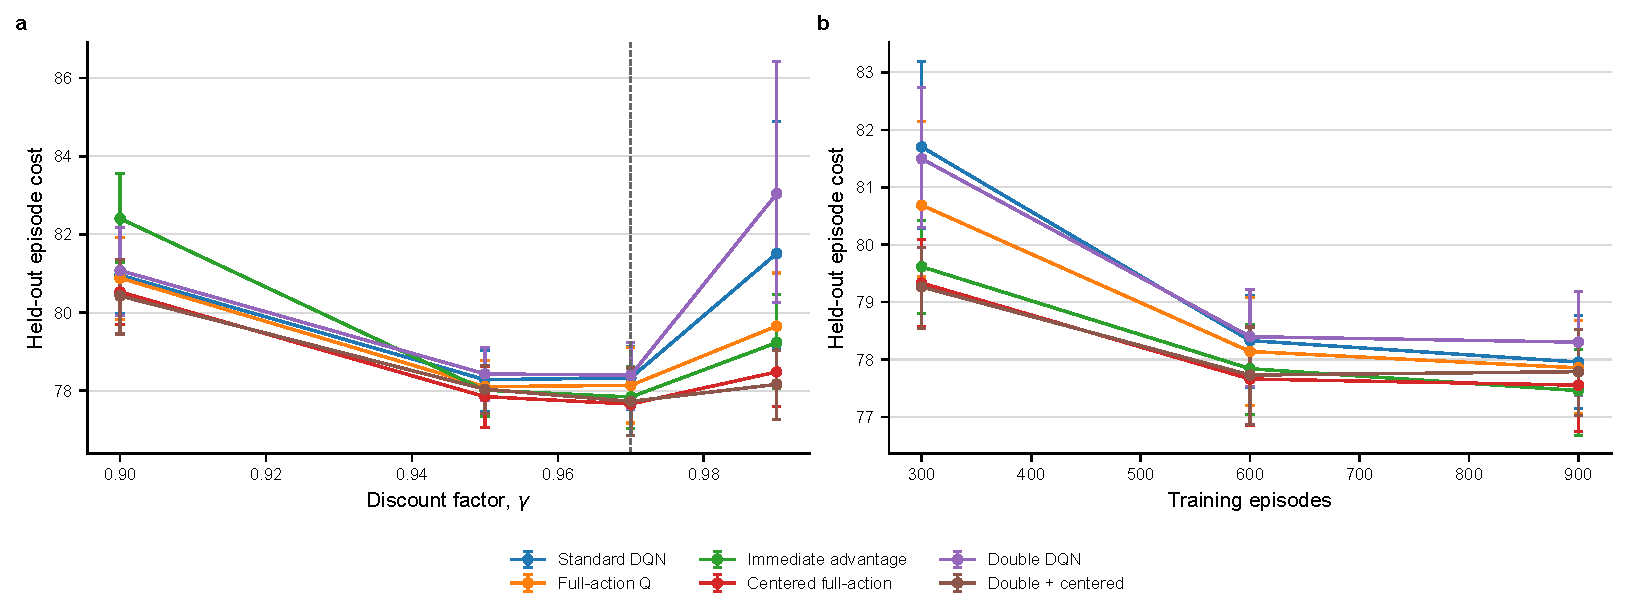
\includegraphics[width=0.98\textwidth]{figures/fig_revision_sensitivity.pdf}
\caption{Nominal sensitivity of all six DQN objectives. (a) Discount-factor sensitivity after 600 training episodes. (b) Held-out episode cost at 300, 600, and 900 training episodes with epsilon decay fixed at 13,440 interactions. Points show means across 20 model-seed blocks after averaging 20 shared traces; bars show 95\% seed-block bootstrap intervals.}
\label{fig:revision_sensitivity}
\end{figure}

Figure~\ref{fig:revision_sensitivity}b reports held-out checkpoints at episodes 300, 600, and 900. The fixed 13,440-interaction exploration schedule makes this a change in training exposure rather than a simultaneous change in epsilon decay. The 12 checkpoint contrasts form their own Holm family. Raw seed-level values and exact intervals are retained in the reproducibility package.

The 300-episode checkpoint had higher mean cost than the 600-episode checkpoint for all six objectives, by 1.53--3.37, and every contrast remained supported after Holm correction. Extending training from 600 to 900 episodes changed the mean by only $-0.38$ to 0.06. None of these six later-checkpoint contrasts met the combined interval and Holm-adjusted sign-test rule. The common late-episode plateau in Fig.~\ref{fig:training} and the held-out checkpoint results therefore support empirical stabilization by 600 episodes, while additional training produced no consistent family-wide gain.

\subsection{Greedy rollout and matched decision time}

The eight-step greedy rollout uses the same perfect preview information as MPC and replans after executing its first action. Table~\ref{tab:revision_runtime} reports nominal cost and CPU decision time for the six DQN objectives, MPC-4, and this baseline. Timing uses batch size one, one CPU thread, shared state samples, and three post-warm-up repetitions; mean, median, and P95 are reported separately. These measurements expose the information and computation context of the cost comparison rather than establishing a universal deployment ranking.

\begin{table}[H]
\centering
\caption{Nominal greedy-rollout and matched CPU decision-time comparison. DQN rows use the current state only; MPC-4 and greedy rollout receive perfect next-task and link-state previews.}
\label{tab:revision_runtime}
\resizebox{\textwidth}{!}{\begin{tabular}{lrrrr}
\toprule
Policy & Episode cost, mean $\pm$ SD & Mean (ms) & Median (ms) & P95 (ms) \\
\midrule
Standard DQN & 78.33 $\pm$ 1.88 & 0.050 & 0.047 & 0.059 \\
Full-action Q & 78.14 $\pm$ 2.23 & 0.050 & 0.047 & 0.059 \\
Immediate advantage & 77.84 $\pm$ 1.82 & 0.051 & 0.047 & 0.064 \\
Centered full-action & 77.66 $\pm$ 1.84 & 0.051 & 0.047 & 0.062 \\
Double DQN & 78.40 $\pm$ 1.98 & 0.050 & 0.047 & 0.060 \\
Double + centered & 77.73 $\pm$ 1.99 & 0.051 & 0.047 & 0.064 \\
MPC-4 & 90.83 $\pm$ 1.71 & 4.772 & 4.985 & 5.434 \\
Greedy rollout-8 & 88.79 $\pm$ 2.19 & 2.538 & 2.722 & 3.021 \\
\bottomrule
\end{tabular}
}
\end{table}

The greedy rollout reduced mean cost relative to MPC-4 (88.79 versus 90.83) but remained above all six DQN means (77.66--78.40). Every paired DQN--greedy difference was negative, ranging from $-11.12$ to $-10.39$; all 95\% bootstrap intervals excluded zero and the largest Holm-adjusted sign-test value was 0.000011. Mean DQN decision time was 0.050--0.051~ms, compared with 2.538~ms for greedy rollout and 4.772~ms for MPC-4. These software measurements correspond to approximately 50-fold and 94-fold differences, respectively, relative to a representative 0.051-ms DQN decision.
\end{revisedblock}

\subsection{Sensitivity of the within-family comparison to parameter changes}

\begin{table}[H]
\centering
\caption{Prespecified parameter sensitivity for centered full-action minus standard DQN. Negative differences favor the centered full-action variant; $n=20$ independent paired model seeds in each profile. Holm adjustment covers the eight displayed profiles.}
\label{tab:sensitivity}
\resizebox{0.84\textwidth}{!}{\begin{tabular}{lrrrr}
\toprule
Parameter profile & Mean difference & 95\% interval & Improvement & Holm $p$ \\
\midrule
Reference & -0.67 & [-0.99, -0.39] & 0.85\% & 0.01804 \\
Compute demand $-20\%$ & -0.49 & [-0.78, -0.22] & 0.79\% & 0.01804 \\
Compute demand $+20\%$ & -0.89 & [-1.35, -0.53] & 0.98\% & 0.00322 \\
Input data $-20\%$ & -1.03 & [-1.55, -0.62] & 1.66\% & 0.01804 \\
Input data $+20\%$ & -0.44 & [-0.69, -0.23] & 0.50\% & 0.01804 \\
Energy use $+20\%$ & -0.60 & [-0.98, -0.28] & 0.57\% & 0.01804 \\
Heat load $+20\%$ & -0.67 & [-1.01, -0.40] & 0.86\% & 0.01804 \\
Link capacity $-20\%$ & -0.64 & [-0.96, -0.35] & 0.72\% & 0.01804 \\
\bottomrule
\end{tabular}}
\end{table}

\begin{figure}[H]
\centering
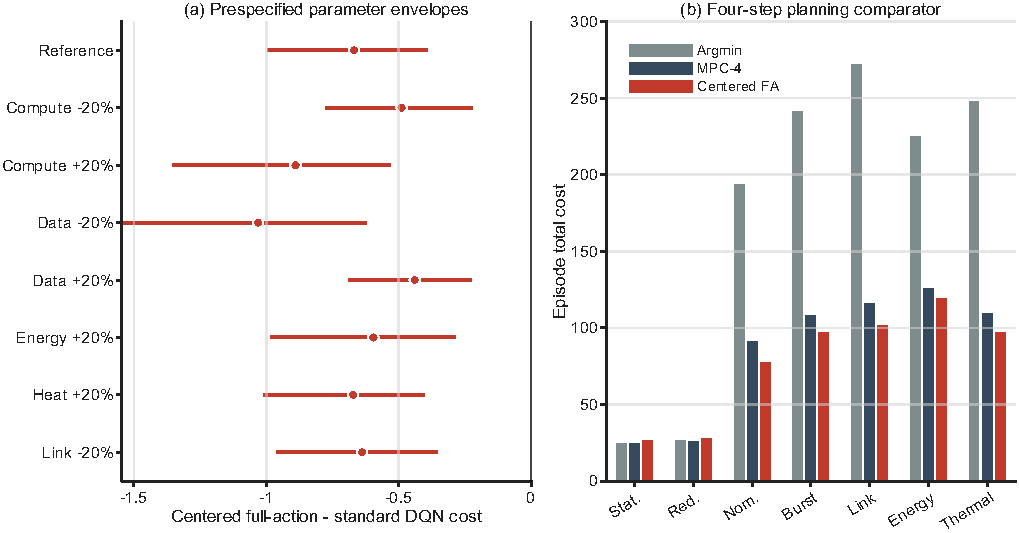
\includegraphics[width=0.98\textwidth]{figures/fig_sensitivity_planning.pdf}
\caption{Parameter sensitivity and planning boundary. (a) Mean paired differences between centered full-action and standard DQN with 95\% paired bootstrap intervals. (b) Immediate, four-step rolling, and learned scheduling across coupling and stress regimes.}
\label{fig:sensitivity}
\end{figure}

The paired interval for centered full-action minus standard DQN remained below zero in all eight profiles. Relative differences ranged from \SensitivityMinPct{} to \SensitivityMaxPct. The largest difference occurred when raw data volume decreased by 20\%, whereas the smallest occurred when it increased by 20\%. The within-family direction therefore remained stable across the prespecified parameter envelope.

\subsection{Preview-scale perturbations bound one model-assisted variant}

\begin{table}[H]
\centering
\caption{Effect of training-time preview misspecification. Differences are relative to the same standard DQN models evaluated in the factual simulator. Scaling applies only to the centered full-action variant's training-time preview cost and action-induced resource changes.}
\label{tab:preview_mismatch}
\resizebox{\textwidth}{!}{\begin{tabular}{llrrrrr}
\toprule
Training preview & Regime & Mean difference & 95\% interval & Negative seeds & Holm $p$ & Supported \\
\midrule
Simulator-exact preview & Nominal & -0.67 & [-0.99, -0.39] & 17/20 & 0.01288 & Yes \\
 & Burst & -0.48 & [-0.73, -0.28] & 17/20 & 0.01288 & Yes \\
 & Link-limited & -0.46 & [-0.77, -0.17] & 15/20 & 0.08278 & No \\
 & Energy-limited & -0.68 & [-1.17, -0.21] & 16/20 & 0.03545 & Yes \\
 & Thermal-stress & -0.45 & [-0.75, -0.22] & 15/20 & 0.08278 & No \\
\addlinespace
Consequences scaled to 0.85 & Nominal & -0.45 & [-0.85, -0.12] & 18/20 & 0.002012 & Yes \\
 & Burst & -0.41 & [-0.72, -0.18] & 17/20 & 0.01031 & Yes \\
 & Link-limited & -0.37 & [-0.62, -0.13] & 13/20 & 0.5264 & No \\
 & Energy-limited & -0.27 & [-0.71, 0.14] & 13/20 & 0.5264 & No \\
 & Thermal-stress & -0.37 & [-0.70, -0.10] & 16/20 & 0.03545 & Yes \\
\addlinespace
Consequences scaled to 1.15 & Nominal & -0.77 & [-1.11, -0.49] & 20/20 & 9.537e-06 & Yes \\
 & Burst & -0.48 & [-0.74, -0.29] & 19/20 & 0.0001602 & Yes \\
 & Link-limited & -0.33 & [-0.62, -0.06] & 13/20 & 0.2632 & No \\
 & Energy-limited & -0.92 & [-1.45, -0.46] & 17/20 & 0.00773 & Yes \\
 & Thermal-stress & -0.42 & [-0.71, -0.18] & 15/20 & 0.08278 & No \\
\bottomrule
\end{tabular}}
\end{table}

Uniform 15\% under- and over-scaling retained favorable mean differences between centered full-action and standard DQN (Table~\ref{tab:preview_mismatch}). The two conditions met the complete support rule in \MismatchLowSupportedCount{} and \MismatchHighSupportedCount{} regimes, respectively. Their largest Holm-adjusted sign-test values were \MismatchLowHolmPMax{} and \MismatchHighHolmPMax.

\section{Discussion}

Six DQN objectives retained a common advantage over MPC-4 across changes in supervision, centering, bootstrapping, and Double DQN evaluation. Their narrow internal spread suggests that the shared sequential value-learning formulation contributed more to performance than the specific target design.

The contextual bandit comparison and planning-depth analysis support a temporal interpretation of this result. The DQN family achieved lower episode costs than immediate-reward learning, while deeper exact enumeration progressively narrowed the cost gap. Together, these observations are consistent with learned values capturing consequences that persist beyond the current allocation.

\begin{revisedblock}
The perfect-forecast MPC results are an optimistic planning reference. Forecast errors can change the selected action sequence and would generally reduce the value of finite-horizon look-ahead, potentially widening the gap to a current-state DQN policy. The magnitude and even the ordering cannot be inferred from uniform noise alone because task-arrival, contact, and structural dynamics errors affect actions differently. A defensible imperfect-MPC comparison therefore requires forecast distributions calibrated to mission data; the present results do not quantify this case.
\end{revisedblock}

The benchmark also makes this comparison traceable and reusable. Shared task primitives generate heat, energy, latency, and transmitted volume, while transition audits connect analytical previews to executed outcomes. Scripts link checkpoints and seed-level estimates to tables, figures, and validation hashes. This evidence chain provides a reproducible platform for comparing sequential decision objectives.

\begin{revisedblock}
The additional nominal tests delimit the robustness claim. Discount-factor and training-length results indicate whether the ordering depends on one value horizon or one stopping point, while the greedy rollout and matched timing results expose the cost of giving a planner perfect previews. They do not establish superiority over MILP, dynamic programming, PPO, SAC, or mission-certified schedulers, which optimize different formulations and feasibility assumptions.
\end{revisedblock}

These findings complement work on simulated experience, model-based acceleration, and action-gap learning~\cite{sutton1991dyna,gu2016continuous,bellemare2016gap}. The evaluated full-action variants use analytical one-step outcomes as auxiliary labels rather than inserting simulated transitions into replay. However, factual-only DQN controls also shared the family-level advantage. The evidence therefore supports long-horizon value learning but does not attribute the advantage to one model-assisted supervision mechanism.

\subsection{Scope and limitations}

\begin{revisedblock}
The scope of these conclusions reflects the use of a synthetic simulator with fixed dimensionless utilities and clipped, soft-constrained resource states; mission-level applicability therefore remains to be assessed. In an operational system, hard energy and thermal envelopes can mask actions, reject tasks, or trigger protective shutdown. Such feasibility changes can reverse the ordering even when a soft-penalty score favors DQN. All learned policies were trained at $c=1$, while the reduced-coupling evaluations jointly vary dynamics and reward scaling. The planner comparison uses perfect forecasts, and the new runtime experiment still compares software implementations rather than flight-qualified processors. Within-family comparisons use an auxiliary weight calibrated for the centered objective, so the individual contributions of centering and bootstrapping remain descriptive rather than factorially identified. Preview misspecification was examined using uniform $\pm15\%$ scaling, which tests amplitude error but not structural error such as an incorrect thermal recurrence, unmodeled actuator saturation, or state-dependent contact loss. More realistic misspecification requires calibrated telemetry, held-out dynamics, and closed-loop hardware-in-the-loop tests. These considerations define the scope of the present benchmark and motivate mission-calibrated validation, while the paired comparative result remains supported under the evaluated conditions.
\end{revisedblock}

\subsection{Future work}

Operational validation should replace fixed dimensionless weights with mission-derived utilities and physical resource dynamics. Action masking, constrained reinforcement learning, and terminal resource conditions can enforce feasibility. Telemetry and hardware-in-the-loop traces can then test whether the observed ordering persists. Multi-satellite, multi-ground-station, and variable-contact topologies can assess scalability.

Mechanism studies should tune auxiliary weights by objective, normalize gradient contributions, and factorially separate centering, Bellman bootstrapping, and discounting. They should also vary transition carryover and delayed-penalty scaling independently. Regime-specific retraining can complement the current $c=1$ transfer tests. Structural, state-dependent, and action-specific preview errors can reveal which components sustain the observed pattern. Family-wide action-mixture analyses can provide complementary evidence.

\begin{revisedblock}
A broader comparator frontier should include scalable tree search, dynamic programming, mixed-integer optimization, PPO, SAC, and satellite-specific schedulers. These methods should be evaluated under matched information and computation budgets, with hard constraints enforced rather than penalized after clipping. Structural model errors should be generated from alternate thermal and energy dynamics, action-specific transition delays, and forecast distributions fitted to telemetry. Decision latency and energy should also be measured on a common flight-like deployment path. Such studies can assess whether the benchmark ordering transfers to operational scheduling.
\end{revisedblock}

\section{Conclusions}

\begin{revisedblock}
The results support a DQN-family advantage within the specified reproducible, resource-coupled benchmark with clipped, soft-constrained resources. All \DQNvsMPCContrastCount{} paired objective--regime contrasts favored DQN over MPC-4, with a family-wide simultaneous 95\% upper bound of \DQNvsMPCGlobalUpperBound. Discount-factor, training-length, greedy-rollout, and matched CPU analyses quantify the stability and computational context of this result. Differences among DQN objectives were smaller and scenario dependent. Hard energy and thermal limits, structural model errors, real mission data, and broader optimization baselines remain outside the evidence boundary, so the result should not be interpreted as universal DQN superiority.
\end{revisedblock}

\authorcontributions{Conceptualization, B.Y.; methodology, B.Y.,L.Z.,D.L.; software, B.Y.,D.L.; validation, B.Y.; formal analysis, B.Y.; investigation, B.Y.; resources, B.Y.,D.L.; data curation, B.Y.; writing---original draft preparation, B.Y.; writing---review and editing, B.Y.; visualization, B.Y.; supervision, B.C.,J.L.; project administration, B.C.,J.L.; funding acquisition, B.C.,J.L. All authors have read and agreed to the published version of the manuscript.}

\funding{This work was supported in part by the National Key Research and Development Program of China under Grants 2022YFF0503904 and 2022YFD2401202; in part by the Shenzhen Higher Education Institutions Stabilization Support Program under Grant GXWD\allowbreak20220811163556003; in part by the National Natural Science Foundation of China under Grants 62202127 and U23A20280; in part by the Shenzhen Science and Technology Program under Grants JCYJ\allowbreak20241202123731040, ZDCY\allowbreak20250901111401002, ZDCY\allowbreak20250901111500001, and ZDCY\allowbreak20250901105202003; in part by the Guangxi Science and Technology Base and Talent Special Project under Grants Gui Ke AD25069103 and Gui Ke DHKL2413 (Research and Application of Key Technologies for Precise Navigation); in part by the Low-Altitude Airspace Strategic Program Portfolio under Grant Z25306106; and in part by the Guangdong Provincial Key R\&D Program under Grant 2026B0909050003.}

\dataavailability{\revised{The public reproducibility package contains the simulator, 1,020 trained checkpoints and corresponding training curves, locked raw evaluations, seed-level summaries, and the bootstrap and Holm-adjusted inference used in this article. It covers the original six-objective benchmark and contextual-bandit comparison, the preview-error and parameter-sensitivity analyses, and the new discount-factor, training-length, eight-step greedy-rollout, and matched decision-time experiments. The repository also provides transition audits, Python and MATLAB reporting source, machine-readable metadata, a complete manifest, and SHA-256 checksums; regenerated outputs are written outside the locked result directories. Pre-rendered manuscript figures and LaTeX source are excluded. The exact code-and-data version used for this revision is commit \texttt{3076c7949333ebcb36643fc5b011ff9db05f78dd} at \url{https://github.com/noob32123/dqn_family_satellite_ground}.}}

\acknowledgments{During the preparation of this manuscript, the authors used OpenAI GPT-5.6-Sol for English-language polishing. The authors reviewed and edited the output and take full responsibility for the content of this publication.}

\conflictsofinterest{The authors declare no conflicts of interest.}

\begin{adjustwidth}{-\extralength}{0cm}
\reftitle{References}
\bibliography{ref}
\PublishersNote{}
\end{adjustwidth}

\end{document}
